% Options for packages loaded elsewhere
\PassOptionsToPackage{unicode}{hyperref}
\PassOptionsToPackage{hyphens}{url}
%
\documentclass[
  man,floatsintext]{apa6}
\usepackage{amsmath,amssymb}
\usepackage{iftex}
\ifPDFTeX
  \usepackage[T1]{fontenc}
  \usepackage[utf8]{inputenc}
  \usepackage{textcomp} % provide euro and other symbols
\else % if luatex or xetex
  \usepackage{unicode-math} % this also loads fontspec
  \defaultfontfeatures{Scale=MatchLowercase}
  \defaultfontfeatures[\rmfamily]{Ligatures=TeX,Scale=1}
\fi
\usepackage{lmodern}
\ifPDFTeX\else
  % xetex/luatex font selection
\fi
% Use upquote if available, for straight quotes in verbatim environments
\IfFileExists{upquote.sty}{\usepackage{upquote}}{}
\IfFileExists{microtype.sty}{% use microtype if available
  \usepackage[]{microtype}
  \UseMicrotypeSet[protrusion]{basicmath} % disable protrusion for tt fonts
}{}
\makeatletter
\@ifundefined{KOMAClassName}{% if non-KOMA class
  \IfFileExists{parskip.sty}{%
    \usepackage{parskip}
  }{% else
    \setlength{\parindent}{0pt}
    \setlength{\parskip}{6pt plus 2pt minus 1pt}}
}{% if KOMA class
  \KOMAoptions{parskip=half}}
\makeatother
\usepackage{xcolor}
\usepackage{graphicx}
\makeatletter
\def\maxwidth{\ifdim\Gin@nat@width>\linewidth\linewidth\else\Gin@nat@width\fi}
\def\maxheight{\ifdim\Gin@nat@height>\textheight\textheight\else\Gin@nat@height\fi}
\makeatother
% Scale images if necessary, so that they will not overflow the page
% margins by default, and it is still possible to overwrite the defaults
% using explicit options in \includegraphics[width, height, ...]{}
\setkeys{Gin}{width=\maxwidth,height=\maxheight,keepaspectratio}
% Set default figure placement to htbp
\makeatletter
\def\fps@figure{htbp}
\makeatother
\setlength{\emergencystretch}{3em} % prevent overfull lines
\providecommand{\tightlist}{%
  \setlength{\itemsep}{0pt}\setlength{\parskip}{0pt}}
\setcounter{secnumdepth}{-\maxdimen} % remove section numbering
% Make \paragraph and \subparagraph free-standing
\ifx\paragraph\undefined\else
  \let\oldparagraph\paragraph
  \renewcommand{\paragraph}[1]{\oldparagraph{#1}\mbox{}}
\fi
\ifx\subparagraph\undefined\else
  \let\oldsubparagraph\subparagraph
  \renewcommand{\subparagraph}[1]{\oldsubparagraph{#1}\mbox{}}
\fi
\newlength{\cslhangindent}
\setlength{\cslhangindent}{1.5em}
\newlength{\csllabelwidth}
\setlength{\csllabelwidth}{3em}
\newlength{\cslentryspacingunit} % times entry-spacing
\setlength{\cslentryspacingunit}{\parskip}
\newenvironment{CSLReferences}[2] % #1 hanging-ident, #2 entry spacing
 {% don't indent paragraphs
  \setlength{\parindent}{0pt}
  % turn on hanging indent if param 1 is 1
  \ifodd #1
  \let\oldpar\par
  \def\par{\hangindent=\cslhangindent\oldpar}
  \fi
  % set entry spacing
  \setlength{\parskip}{#2\cslentryspacingunit}
 }%
 {}
\usepackage{calc}
\newcommand{\CSLBlock}[1]{#1\hfill\break}
\newcommand{\CSLLeftMargin}[1]{\parbox[t]{\csllabelwidth}{#1}}
\newcommand{\CSLRightInline}[1]{\parbox[t]{\linewidth - \csllabelwidth}{#1}\break}
\newcommand{\CSLIndent}[1]{\hspace{\cslhangindent}#1}
\ifLuaTeX
\usepackage[bidi=basic]{babel}
\else
\usepackage[bidi=default]{babel}
\fi
\babelprovide[main,import]{english}
% get rid of language-specific shorthands (see #6817):
\let\LanguageShortHands\languageshorthands
\def\languageshorthands#1{}
% Manuscript styling
\usepackage{upgreek}
\captionsetup{font=singlespacing,justification=justified}

% Table formatting
\usepackage{longtable}
\usepackage{lscape}
% \usepackage[counterclockwise]{rotating}   % Landscape page setup for large tables
\usepackage{multirow}		% Table styling
\usepackage{tabularx}		% Control Column width
\usepackage[flushleft]{threeparttable}	% Allows for three part tables with a specified notes section
\usepackage{threeparttablex}            % Lets threeparttable work with longtable

% Create new environments so endfloat can handle them
% \newenvironment{ltable}
%   {\begin{landscape}\centering\begin{threeparttable}}
%   {\end{threeparttable}\end{landscape}}
\newenvironment{lltable}{\begin{landscape}\centering\begin{ThreePartTable}}{\end{ThreePartTable}\end{landscape}}

% Enables adjusting longtable caption width to table width
% Solution found at http://golatex.de/longtable-mit-caption-so-breit-wie-die-tabelle-t15767.html
\makeatletter
\newcommand\LastLTentrywidth{1em}
\newlength\longtablewidth
\setlength{\longtablewidth}{1in}
\newcommand{\getlongtablewidth}{\begingroup \ifcsname LT@\roman{LT@tables}\endcsname \global\longtablewidth=0pt \renewcommand{\LT@entry}[2]{\global\advance\longtablewidth by ##2\relax\gdef\LastLTentrywidth{##2}}\@nameuse{LT@\roman{LT@tables}} \fi \endgroup}

% \setlength{\parindent}{0.5in}
% \setlength{\parskip}{0pt plus 0pt minus 0pt}

% Overwrite redefinition of paragraph and subparagraph by the default LaTeX template
% See https://github.com/crsh/papaja/issues/292
\makeatletter
\renewcommand{\paragraph}{\@startsection{paragraph}{4}{\parindent}%
  {0\baselineskip \@plus 0.2ex \@minus 0.2ex}%
  {-1em}%
  {\normalfont\normalsize\bfseries\itshape\typesectitle}}

\renewcommand{\subparagraph}[1]{\@startsection{subparagraph}{5}{1em}%
  {0\baselineskip \@plus 0.2ex \@minus 0.2ex}%
  {-\z@\relax}%
  {\normalfont\normalsize\itshape\hspace{\parindent}{#1}\textit{\addperi}}{\relax}}
\makeatother

% \usepackage{etoolbox}
\makeatletter
\patchcmd{\HyOrg@maketitle}
  {\section{\normalfont\normalsize\abstractname}}
  {\section*{\normalfont\normalsize\abstractname}}
  {}{\typeout{Failed to patch abstract.}}
\patchcmd{\HyOrg@maketitle}
  {\section{\protect\normalfont{\@title}}}
  {\section*{\protect\normalfont{\@title}}}
  {}{\typeout{Failed to patch title.}}
\makeatother

\usepackage{xpatch}
\makeatletter
\xapptocmd\appendix
  {\xapptocmd\section
    {\addcontentsline{toc}{section}{\appendixname\ifoneappendix\else~\theappendix\fi\\: #1}}
    {}{\InnerPatchFailed}%
  }
{}{\PatchFailed}
\keywords{L3 acquisition, L3 perception, replication\newline\indent Word count: X}
\usepackage{lineno}

\linenumbers
\usepackage{csquotes}
\ifLuaTeX
  \usepackage{selnolig}  % disable illegal ligatures
\fi
\IfFileExists{bookmark.sty}{\usepackage{bookmark}}{\usepackage{hyperref}}
\IfFileExists{xurl.sty}{\usepackage{xurl}}{} % add URL line breaks if available
\urlstyle{same}
\hypersetup{
  pdftitle={The double phonemic boundary effect at L3 ab-initio},
  pdfauthor={Kyle Parrish1},
  pdflang={en-EN},
  pdfkeywords={L3 acquisition, L3 perception, replication},
  hidelinks,
  pdfcreator={LaTeX via pandoc}}

\title{The double phonemic boundary effect at L3 ab-initio}
\author{Kyle Parrish\textsuperscript{1}}
\date{}


\shorttitle{L3 DPBE}

\authornote{

Correspondence concerning this article should be addressed to Kyle Parrish, Theodor-W.-Adorno-Platz 1, 60629 Frankfurt am Main. E-mail: \href{mailto:parrish@em.uni-frankfurt.de}{\nolinkurl{parrish@em.uni-frankfurt.de}}

}

\affiliation{\vspace{0.5cm}\textsuperscript{1} Goethe University Frankfurt}

\abstract{%
The present study was an approximate replication of Rothman (2011) and examined the determiner phrase (DP) syntax of a large sample (n = 211) of L3 learners of Portuguese who spoke English and Spanish.
Rothman (2011) investigated whether L3 Italian or Brazilian Portuguese speakers would be differently impacted by another known Romance Language if it was their L1 or L2.
The original study concluded that groups did not perform differently on the experimental tasks on the basis of a null effect, and that the typological similarity of Spanish and Portuguese or Italian, relative to English, predicts transfer in the initial stages of L3 acquisition.
The present replication recreated all materials, which were not available, but examined the same population and questions.
Rather than examining L3 Italian and L3 Brazilian Portuguese, the present work maintained a constant L3, Portuguese
The learners were divided into two groups in a mirror-image design (n = 96 L1 English-L2 Spanish, n = 115 L1 Spanish-L2 English) and data was collected completely online.
Like the original study, there was not a main effect of group in any of the two-way Analyses of Variance.
However, these results show that it should not be assumed that experimental groups behave equivalently based on a null effect: out of four total post-hoc tests of equivalence, only two were significant when the equivalence bounds were set at a small effect size (d = +/- .4).
Ultimately, it is argued that determining the smallest effect size of interest and subsequent equivalence testing are necessary to answer key questions in the field of L3 acquisition.
}



\begin{document}
\maketitle

\hypertarget{introduction}{%
\section{Introduction}\label{introduction}}

The endeavor of learning an additional language during adulthood is difficult.
This is especially true when one considers phonological acquisition.
For instance, numerous studies over the course of the past five decades have demonstrated that adult second language (L2) learners often produce and perceive the sounds of the target language in a non-native manner (Bohn \& Flege, 1993; Flege \& Eefting, 1987; \textbf{flege\_cross?}).
This difficulty arises, in part, because bilinguals often navigate complex communicative situations in which they produce and perceive speech from both of their languages in real time.
Recent studies suggest that bilinguals learn to modify their perceptual categorization routines in accordance with the phonetic realizations of the language they believe they are hearing (Casillas \& Simonet, 2018; Gonzales et al., 2019; Gonzales \& Lotto, 2013; Lozano-Argüelles et al., 2020).
Much less is known about the acquisition of a third language (L3A), particularly with regard to L3 production, perception, and phonological learning.
The present investigation explores the perceptual categorization routines of adult bilinguals during the initial stages of L3 acquisition.

Fields such as third language acquisition and bilingual phonology can provide a compelling example that interdisciplinary work can be mutually beneficial.
For instance, the field of third language (L3) acquisition has a primary goal of determining how the two languages known by a bilingual influence the learning of a third language (Cabrelli Amaro \& Wrembel, 2016).
In order to determine whether L3 performance can be attributed to the influence of a single language, it is necessary to conceive of these languages as being separate to some degree.
The degree of separation of language systems has also been debated in bilingual phonology, where it is argued that second language (L2) learners are able to form L2 specific phonological categories in the process of acquisition (Simonet, 2016).
Taken together, the debates in L3A and L2 phonology can inform one another if it could be determined that L3 behavior can be reasonably likened to either L1 or L2 behavior.
If this result were to be found, it would simultaneously be evidence of separate phonological systems in bilinguals and it would inform L3 models' debates on the source language of influence in L3 acquisition.

Research in L2 phonology has argued that language specific categories, while related to L1 categories, emerge as proficiency increases and are dictated by context.
This idea of context was further conceptualized by Grosjean in the idea of bilingual language modes which exist on a continuum (Grosjean, 1989).
In this view, bilinguals have two possible unilingual modes in either of their languages, in which they expect to perceive and produce only one language.
However, bilinguals often find themselves in a situation in which the use of both languages is plausible.
This dynamic phenomenon of language mode is thought to have an effect on a bilingual speakers categorization of sounds, in which a bilingual would display more monolingual like behavior in a unilingual mode, and evidence increased crosslinguistic interactions in a bilingual mode.
The perspective of bilingual language modes has not been considered by L3 models, which either posit that a single language influences the L3 entirely (Bardel \& Falk, 2012; Rothman, 2015), or that structure by structure influence is possible (Slabakova, 2017; Westergaard et al., 2017).

Broadly, L3 models which predict single language influence vary in their predictions of which language known by the bilingual influences L3 acquisition. On one hand, it has been suggested that the second language learned by a late bilingual (after the age of 12) is the default source of influence (Bardel \& Falk, 2012).
On the other, typological similarity has been suggested as a the driving factor that allows for either first or second language influence of the L3, but not both (Rothman, 2015).
These full transfer models of L3 acquisition have distinct cognitive motivations which fuel their predictions, which may be at odds with some perspectives in L2 phonology.
For example, it has been argued that single language influence is more cognitively economical than structure by structure transfer (Rothman, 2015).
However, if language sound systems are dynamic and may become more or less integrated depending upon the patterns of particular language use, it is difficult to argue that a bilingual will behave using language specific and independent categories at all times.
From this point of view, the language mode of a bilingual when they encounter a third language is vital, since it is possible that the L3 may be associated with a particular language that a bilingual knows and result in L3 processing in that language specific mode.

The idea that bilingual sound systems are sensitive to the linguistic context is one of the notions which motivated the so-called language set experiments
(Caramazza et al., 1973; Caramazza \& Yeni-Komshian, 1974; Casillas \& Simonet, 2018; Flege \& Eefting, 1987; Gonzales et al., 2019; Gonzales \& Lotto, 2013; Lozano-Argüelles et al., 2020; Williams, 1977).
This literature is interested in how bilinguals categorize sounds in language specific modes, and attempted to place bilinguals in unilingual modes in each of their languages to demonstrate that bilinguals show evidence of having two separate language specific perceptual routines.
Focusing on the contrast between /p/ and /b/, these studies would present participants with a continuum of sounds (one at a time) and a two alternative forced choice task (2afc), where each given sound was categorized as either /p/ or /b/.
Importantly, the continua were presented twice to the same participant, once in which they were told that it was one language (say, English) and a second time when they were told it was a different languages.
The results showed that the perceptual boundary shifted in the expected direction, even when there were no acoustic differences in the stops themselves, as a function of the language that the participants believed they were hearing.
This effect is referred to in the literature as the double phonemic boundary effect (Casillas \& Simonet, 2018; Gonzales \& Lotto, 2013; Lozano-Argüelles et al., 2020), in which a bilingual shows evidence of two possible categorizations of the same sound on the basis of the language in which it is uttered.

In the case of stop consontants, the continua used in studies has varied by voice onset time (VOT).
VOT refers to the time interval between the release of a stop consonant and the onset of vocal fold vibration (Lisker \& Abramson, 1964).
For example, in Spanish, the difference between {[}p{]} and {[}b{]} is manifested as a difference in VOT.
Where {[}b{]} is voiced (a negative VOT), {[}p{]} is voiceless (a positive VOT).
Languages which contain this distinction, in which the realizations of /p/ and /b/ are phonetically voiceless and phonetically voiced, respectively, are referred to as ``true-voicing languages'' (Lisker \& Abramson, 1964).
Relevant to the present study, Spanish, French, and Hungarian fall under this category.
English, on the other hand, contrasts stop consonants with only positive VOT via a long versus short lag distinction.
As a result, previous studies have shown that the perceptual boundary between /p/ and /b/ in what is believed to be Spanish occurs at a higher VOT value than the boundary between /p/ and /b/ in English.

The present work employs and adapts the methods of recent studies which found a double phonemic boundary effect in bilinguals to test the predictions of third language (L3) models of morphosyntax and shed light on whether perceptual boundaries in a third language are L1-like, L2-like, or intermediate of the L1 and L2 boundary.
In order to do so, Spanish-English bilingual speakers categorized the same /p/-/b/ VOT continua under the guise that it was four distinct languages, English, Spanish, French and Hungarian.
English and Spanish were included to determine whether the speakers had unique perceptual boundaries, and as a result provide evidence that their new language categorizations was L1 or L2-like.
The new languages were chosen to examine whether psychotypological effects would be seen in perception.
That is, French was chosen based historical relationship with Spanish with the idea that participants would categorize French similarly to Spanish, while Hungarian was chosen for its unclear relationship with English or Spanish.

Vitally, bilinguals, rather than L3 learners, were chosen for this experiment because the goal was to inform how L3 learners perceive and categorize sounds in their to-be third language in the very early stages of learning, and whether this perception is modulated by the perceptual routines in one of their known languages.
Additionally, by using participants who do not yet have knowledge of a third language, the confound of acquisition and L1 or L2 influence is far less likely.
That is, if the present study found a given L3 perceptual boundary in more advanced L3 learners, it could not be determined whether this boundary is simply their acquired L3 perceptual routine on the basis of their experience in the L3 itself, and not the influence of their L1 or L2 boundaries.
To reiterate, the principal question of the present work is how bilingual speakers perceive a new language when they already have two language specific perceptual boundaries.
In general, these cross-linguistic relationships allow for the testing of the predictions of L3 models of morphosyntax and their extension to L3 perception.

\hypertarget{previous-work-in-the-double-phonemic-boundary-effect}{%
\subsection{Previous work in the Double Phonemic Boundary Effect}\label{previous-work-in-the-double-phonemic-boundary-effect}}

Past research has yielded mixed results in its attempt to demonstrate that bilinguals have language specific perceptual routines, and that the boundary between language specific categories vary as a function of language mode.
In other words, in this research paradigm, bilinguals are assumed to have language specific categories of sounds (phonemes), which, in theory, should lead to distinct categorizations of the same acoustic stimuli (such as a step on a VOT continuum) as a function of language mode.

An initial series of studies focused on VOT and yielded null results.
These studies examined the categorization of a /p/-/b/ continuum in two languages.
Importantly, this continuum was the same in both sessions, and the hypothesis of these studies was that placing bilinguals in a language specific mode would lead to distinct categorization of the same continuum in two different sessions by the same participant.
In studies of young Canadian French-English bilinguals' perception and productions of three voicing contrasts (Caramazza et al., 1973, 1974), it was found that bilinguals and monolinguals differed in their perceptual boundaries of each language in perception, but that the bilinguals did not categorize the continua differently in English and Spanish.
The authors did, however, report language specific differences in production.
Another study of Spanish-English bilinguals in the United States (Williams, 1977), found participants categorized a /p-b/ VOT continuum the same in both language modes.

By identifying some potential causes of null results in the previous literature, subsequent studies made methodological adjustments and found double phonemic boundary effects in bilinguals that was modulated by language mode.
Elman et al. (1977) maintained the use of the same acoustic continuum between languages, but used naturally produced stimuli, rather than the synthetic continuum used in previous studies (Caramazza et al., 1973, 1974; Williams, 1977).
Additionally, Elman et al. (1977) argued that simply being placed in a language specific mode does not guarantee its maintenance throughout the experimental session.
In order to address this, Elman et al. (1977) added language specific filler words to keep participants in the appropriate language mode.
As a result, a double phonemic boundary effect was observed in the Spanish-English participants.
Further studies found similar effects in the categorizations of a VOT continuum in French-English (Hazan \& Boulakia, 1993) and Dutch-English bilinguals (Flege \& Eefting, 1987)

Subsequent studies examined the role of language proficiency in magnitude of mode effects in bilinguals.
Garcia-Sierra et al. (2009) found that the double phonemic boundary effect in Spanish-English bilinguals was modulated by proficiency, such that the participants with greater self-reported proficiency made wider distinctions between their mode driven categorizations of the VOT continuum used in the study.
Other studies have maintained language mode by using language specific segments within pseudoword stimuli to perceptually cue a particular language mode (Casillas \& Simonet, 2018; Gonzales \& Lotto, 2013). In the original study, Gonzales and Lotto (2013) created a VOT continuum using the pseudowords \emph{pafri} and \emph{bafri} as the choices available in a 2-alternative forced choice task.
The participants heard a rendition of ``parfi'' or ``bafri in both an English and Spanish session.
Rather than language specific filler words, these authors changed the second half of the pseudowords''fri'' so that they contained either an English rhotic or Spanish rhotic in each session of the experiment.
Importantly, the /pa/-/ba/ first syllable of the pseudowords was identical in both sessions, so that the participants were categorizing pseudowords that had an identical range of VOTs, but distinct, language specific rhotic sounds.
The results revealed a double phonemic boundary effect in the Spanish-English bilingual participants with exposure to both languages from early childhood. These results were replicated by Casillas and Simonet (2018), in which the pseudowords pafri-bafri were again used.
The findings extended the double phonemic boundary effect to L2 learners, in which higher proficiency L2 learners of Spanish showed stronger L2 boundary effects.

Two follow up studies also investigated the categorization of word initial stops /b/ and /p/ in Spanish-English bilinguals, and young Spanish-English and French-English bilinguals (Gonzales et al., 2019; Lozano-Argüelles et al., 2020).
Differently from Casillas and Simonet (2018) and Gonzales and Lotto (2013), these studies presented only the first syllable of the pafri-bafri continuum and the onset of the second syllable (paf-baf), and manipulated the participants' language mode using conceptual cueing by telling participants they were listening to English or Spanish sounds, rather than perceptual cueing of the language specific rhotic sounds used by previous studies.
The results were consistent with previous studies; sufficiently proficient L2 Spanish speakers show language mode effects in their categorization of /p/ and /b/ on a VOT continuum, whether this is perceptually or conceptually cued.

\hypertarget{the-present-study}{%
\subsection{The Present Study}\label{the-present-study}}

It is this conceptual cuing which resulted in a double phonemic boundary effect found by Lozano-Argüelles et al. (2020) and Gonzales et al. (2019) that motivates the present study.
Since L3 learners likely detect phonetic cross-linguistic similarities in L3 input, the present study examines the role of conceptual cueing on L3 categorization at the first exposure to L3 input by omitting the presence of language specific segments from the stimuli.
Following the previous literature, which demonstrates that Spanish-English bilinguals categorize the same continuum of sounds differently depending upon the language they believe they are hearing, the present study both replicates these findings in the /p/-/b/ VOT and examines whether one of these boundaries are used to categorize sounds in a new language, unknown to the speaker.
Additionally, the present study is concerned with whether the third language has a well known historical relationship with previously known languages, and if this affects sound categorization.
That is, whether participants who believe they are hearing French will be biased to categorize the continua as similar to their Spanish categorizations.
This bias would be argued to be modulated by a metalinguistic knowledge of cross-linguistic similarity and historical relationship between Spanish and French.
In particular, the present work is guided by the following research questions:

RQ1: Will the double phonemic boundary effect found in previous studies be replicated?

RQ2: Assuming that bilinguals display the same double phonemic boundary demonstrated in previous studies, will their categorizations of what they believe are the L3 continua resemble their categorizations of either their L1 or their L2?

In order to answer the subsequent research questions of this study, it was vital to replicate the findings of previous studies which found a double phonemic boundary effect in stop consonants in Spanish-English bilinguals (Casillas \& Simonet, 2018; Gonzales et al., 2019; Gonzales \& Lotto, 2013; Lozano-Argüelles et al., 2020).
In the event that the perceptual boundaries of just one language are used in L3 perception regardless of whether it is believed to be French or Hungarian, this finding provide evidence that a language specific bias exists. On the other hand, if bilinguals categorize one continuum using the L1 and the other using the L2, it would suggest that the language that L3 speakers believe they are hearing biases their perceptual routines in that language.

\hypertarget{methods}{%
\section{Methods}\label{methods}}

\hypertarget{participants}{%
\subsection{Participants}\label{participants}}

Additionally, participants who failed attention checks, chose the same answer for every trial, or who answered over 80\% /p/ or /b/ in the stops trials were removed from the data analysis.

\hypertarget{materials}{%
\subsection{Materials}\label{materials}}

The experiment was composed of 5 total blocks.
An itemized version of the Language History Questionnaire (Li et al., 2020) was given to participants and asked their first language, second language, and the age at which they began learning their L2.
The measure of L2 proficiency, the lexTALE (Izura et al., 2016; Lemhöfer \& Broersma, 2016), was given in Spanish to the ES group and English to the SE group.
The lexTALE is a lexical decision task in which the participants are presented with either a word or a non-word, and they must decide whether the word presented exists in that language.
Both the Spanish and English versions are scored in the same manner, and allow for comparability of proficiency across groups. Both versions contain 60 words total, 40 of which are real words and 20 of which are non-words. A formula then calculates a score based on the percentage of real words correct plus the percentage of non-words correct divided by 2.

Following these tasks, participants then took a series of three two-alternative forced choice tasks (2afc).
The tasks were programmed in Psychopy (Peirce et al., 2019) and were hosted on Pavlovia.org.
Participants received written instructions prior to taking part in each phase of the experiment. The instructions for the ``English'' task were in English, the instructions for the ``Spanish'' task were in Spanish, and the instructions for the L3 tasks were bilingual (both Spanish and English). In each block, the instructions on prolific were in the language mode that the participants were told that they would hear, and the instructions within the experiment itself were also language specific, with the exception of all L3 prolific instructions being in English. These instructions read ``Final step! You have been assigned to the Hungarian/French group.
The task is the same as the first two sessions, but this time, the words are from the Hungarian/French language.'' In the L3 experimental session, written instructions were more scarce, since the participants had already completed the same procedure twice, but were always presented in both English and Spanish at the same time. Instructions appeared at the beginning of the experiment, after the initial practice trials, and between the stop and vowel sessions, and for the attention checks. In each case, and English instruction was given and its Spanish translation appeared either to the right of the English instruction or immediately below it.
As in previous studies, the instructions contained no instances of the experimental stimuli, in this case ``pafri'', ``bafri,''ifri, or ``ufri'', or any of their language specific forms appeared during the instructions.

\hypertarget{stimuli}{%
\subsection{Stimuli}\label{stimuli}}

The 2afc tested the perception of the same two continua (a /p/-/b/ VOT continuum and a /i/-/u/ F2 continuum) in three different language modes: English, Spanish and the L3 (either Hungarian or French). The VOT continuum has been used in previous studies (Gonzales et al., 2019; Lozano-Argüelles et al., 2020) and were created from a recording by a female Spanish-English bilingual. The original VOT continuum contained the word ``pafri'' and ``bafri''. The recording was resynthesized and ranged in VOT from -35ms to 35ms, excluding a 0 VOT step. In the present study, three additional steps were added on the positive end of the scale in order to increase the chances of /p/ responses at the positive extreme of the continuum, such that steps of 40ms, 45ms, and 50ms were included and made a total of 17 total steps. The extra steps were created manually in PRAAT by extracting 5ms of the voiceless part of the previous segments and adding these portions on to the beginning of the 35ms stimulus up to three times.
Just as in Lozano-Argüelles et al. (2020), the present study conceptually cued participants, and did not utilize the language specific rhotics used in Gonzales and Lotto (2013) and Casillas and Simonet (2018).

During the 2afc task, participants saw both the words \emph{pafri} and \emph{bafri} or language specific versions of \emph{ifri} and \emph{ufri} on the screen and just the first syllable of these words in which the initial consonant was a member of the continuum (``paf'' or ``baf'' for vowels, ``if'' or ``uf'' for vowels).
Each step of the continuum was played 5 times total, leading to a total of 85 trials in the VOT continuum per participant and 55 total trials in the vowel continuum.
Each trial was drawn randomly from the continuum in a single block, so no participant heard the same stimulus order.
Due to language specific orthographic differences, the non-words on screen were distinct orthographically in each language, with the exception of French and Spanish.
In Spanish and French, the participants saw \emph{ifri} and \emph{ufri} on the screen, in English they saw \emph{eefri} and \emph{oofri}, and in Hungarian, they saw \emph{ifrelo} and \emph{ufrelo}. This spelling difference was necessary because of the orthographic conventions in the realizations of similar sounds between English and Spanish. For example, the Spanish grapheme ``u'' and the English graphemes ``oo'' are similar in their acoustic realizations. On the other hand, the choice of spelling in the French and Hungarian stimuli were made to reflect that high degree of lexical overlap between Spanish and French, and to reinforce the ambiguous relationship between Hungarian and English or Spanish.

\hypertarget{procedure}{%
\subsection{Procedure}\label{procedure}}

All participants completed a total of five tasks, the Language History Questionnaire, the lexTALE proficiency test in their L2, and three 2afc tasks. First, the participants completed the Language History Questionnaire online (Li et al., 2020), followed by the lexTALE proficiency test.
Following these two tasks used for screening, only those participants who did have knowledge of a third language and scored at least 60\% on the lexTALE were deemed eligible and continued the experiment. This cutoff was chosen to focus the analysis on more proficient bilinguals, rather than demonstrate that increasing proficiency is correlated to a larger double phonemic boundary effect size, as has been found in previous studies (Casillas \& Simonet, 2018; Garcia-Sierra et al., 2009; Gonzales \& Lotto, 2013).

Following these screening tasks, and in order to control for language mode, the participants completed the 2afc tasks in a semi-longitudinal design.
Participants were invited to take part in the second portion of the experiment at least 30 minutes after their completion of the previous step. In many cases, however, participants completed different blocks of the experiment hours or days apart.
All participants began with the ``English'' task, followed by ``Spanish'', and finished with either ``French'' or ``Hungarian''. Unfortunately, the lack of counterbalancing across participants is a limitation in the design of the current study.
In the English and Spanish tasks, the instructions were given in that respective language, and it was explained that the participants were going to hear rare words in the language in question (English, Spanish or the L3).
In the L3 session, the same instructions were given in both English and Spanish simultaneously and on the same screen in order to avoid biasing the participants to either English or Spanish mode.

\hypertarget{statistical-analyses}{%
\subsection{Statistical analyses}\label{statistical-analyses}}

In order to determine a crossover boundary for each participant in a group model, three logistic regression models were fit to each participant (one for each of three languages), which predicted their responses of `bafri'/`pafri' as a function of step in the VOT continuum.
As a result, 3 crossover boundaries total were calculated per participant that provided which step in the continuum the probability of the participant choosing either ``pafri'' or ``bafri'' was 50\%.
All analyses were carried out in R (R Core Team, 2020) and used either the stats package or the brms packages (\textbf{R-brms?}).

\hypertarget{methods-1}{%
\section{Methods}\label{methods-1}}

We report how we determined our sample size, all data exclusions (if any), all manipulations, and all measures in the study.

\hypertarget{results}{%
\section{Results}\label{results}}

Figure 1 shows the breakdown of participant categorizations.
Half of the participants showed evidence of a DPBE, making them appropriate for subsequent within-subjects analyses.
The 30 participants with no effect were not include in the within subjects-analysis, which was designed to determined which language-specific phonemic boundary is more similar to a novel language's, since their Spanish and English was not distinct (enough) to determine whether their ``L3'' was closer to one or the other.

\begin{figure}
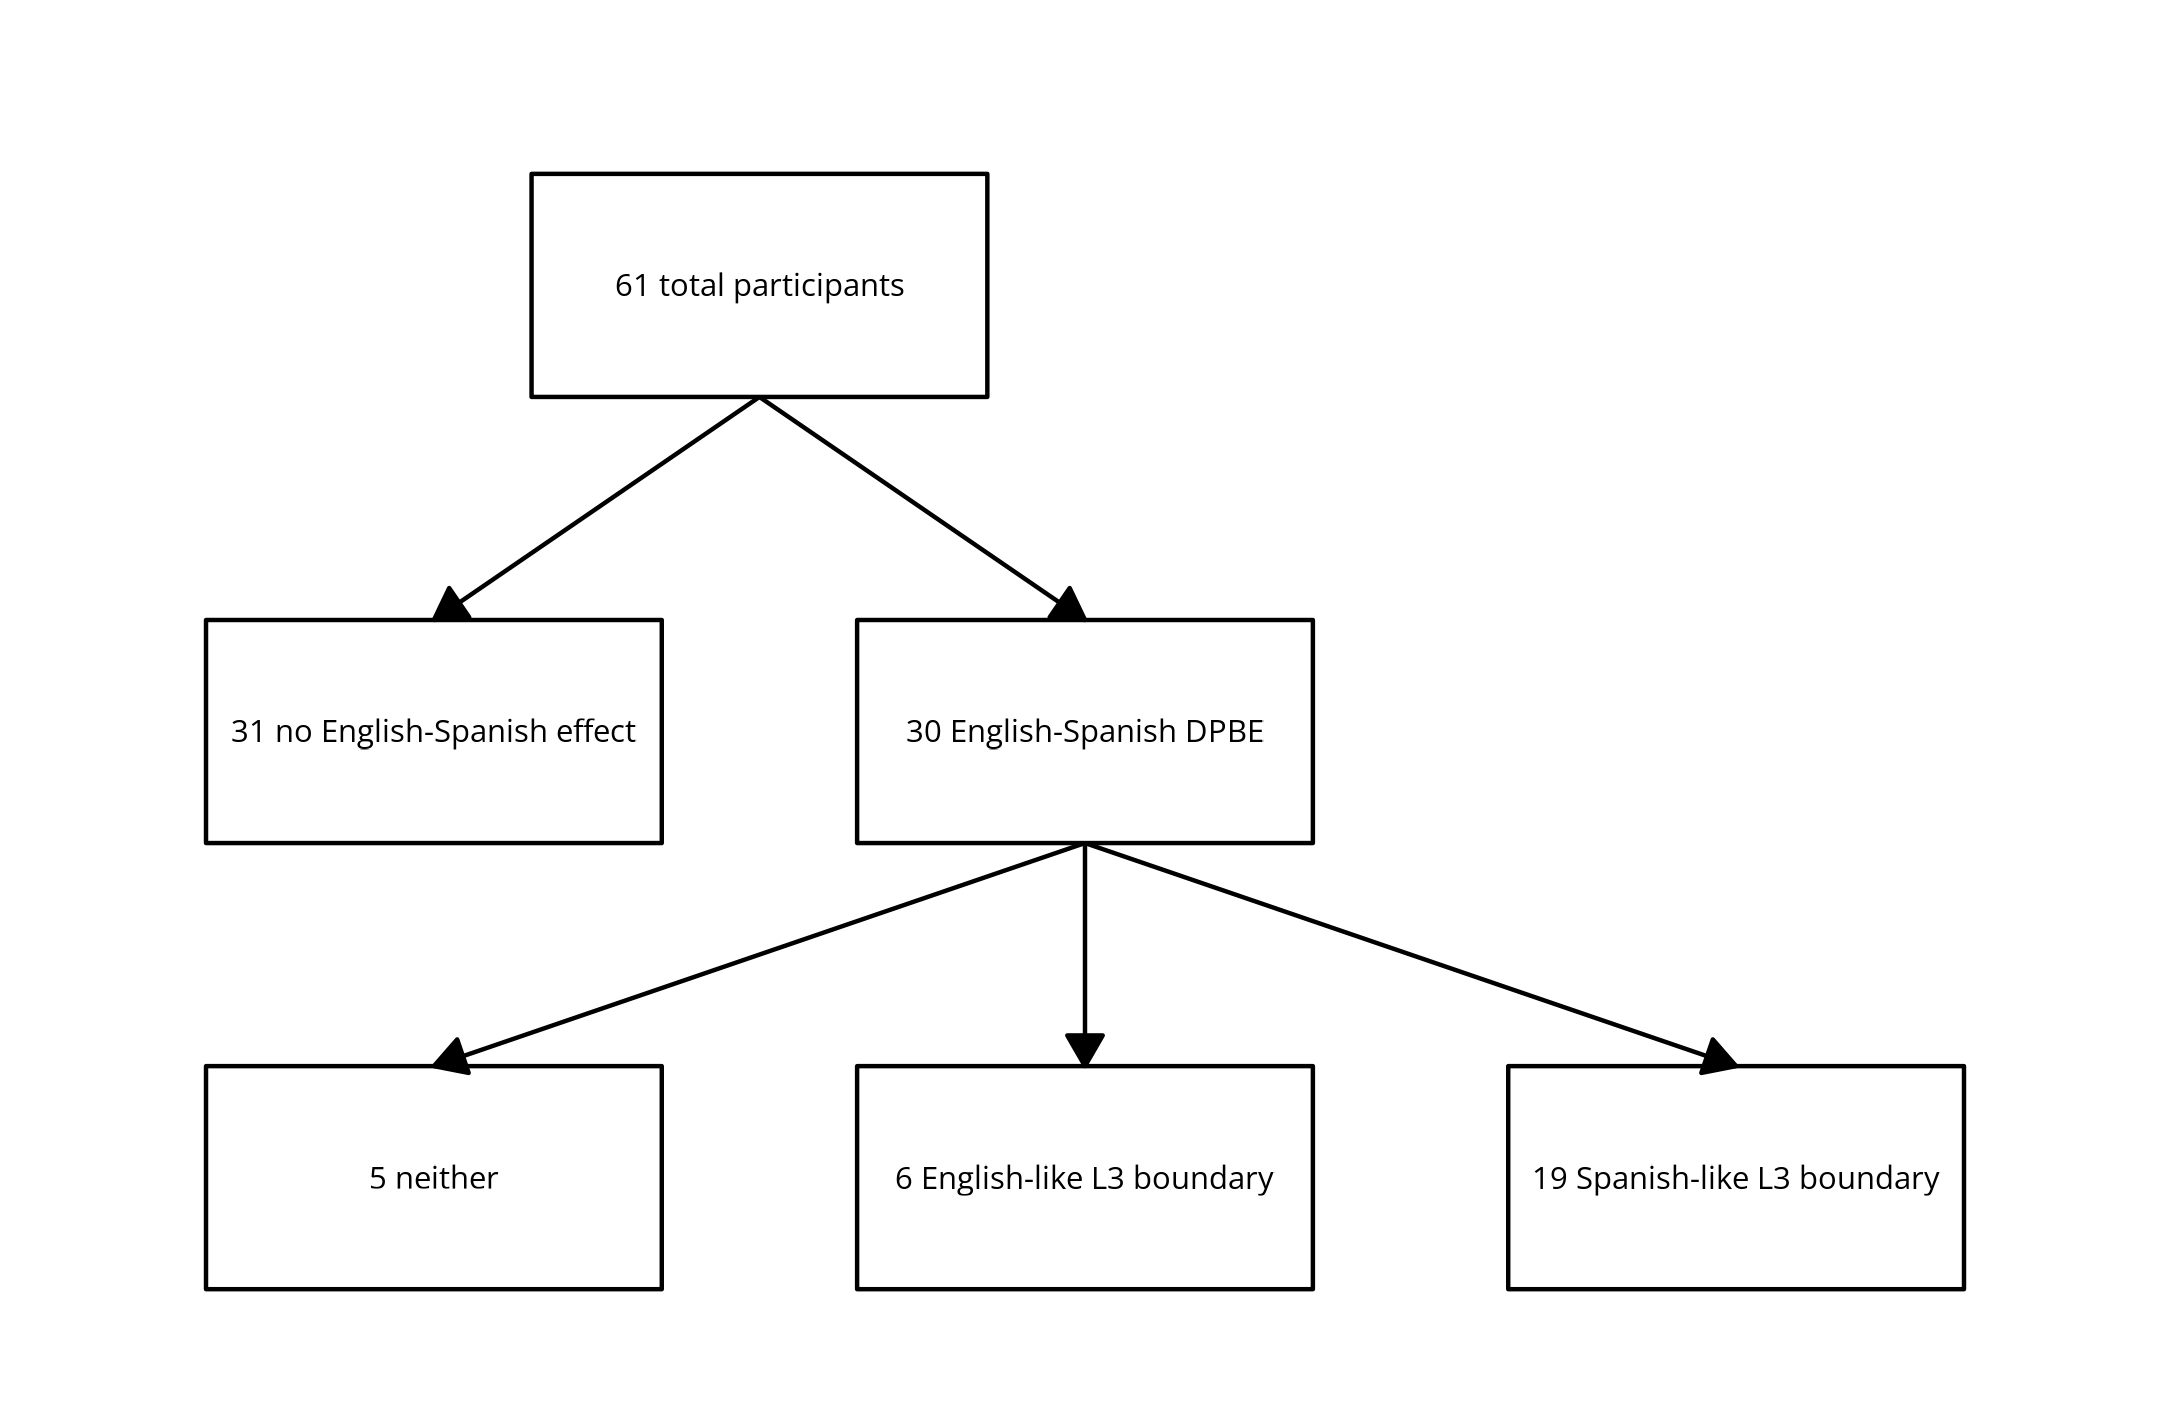
\includegraphics[width=425px]{new_docs/img/flow_chart} \caption{ }\label{fig:unnamed-chunk-1}
\end{figure}

\textbf{Breakdown of L1 and ``L3'' for participants with the DPBE}

\begin{figure}
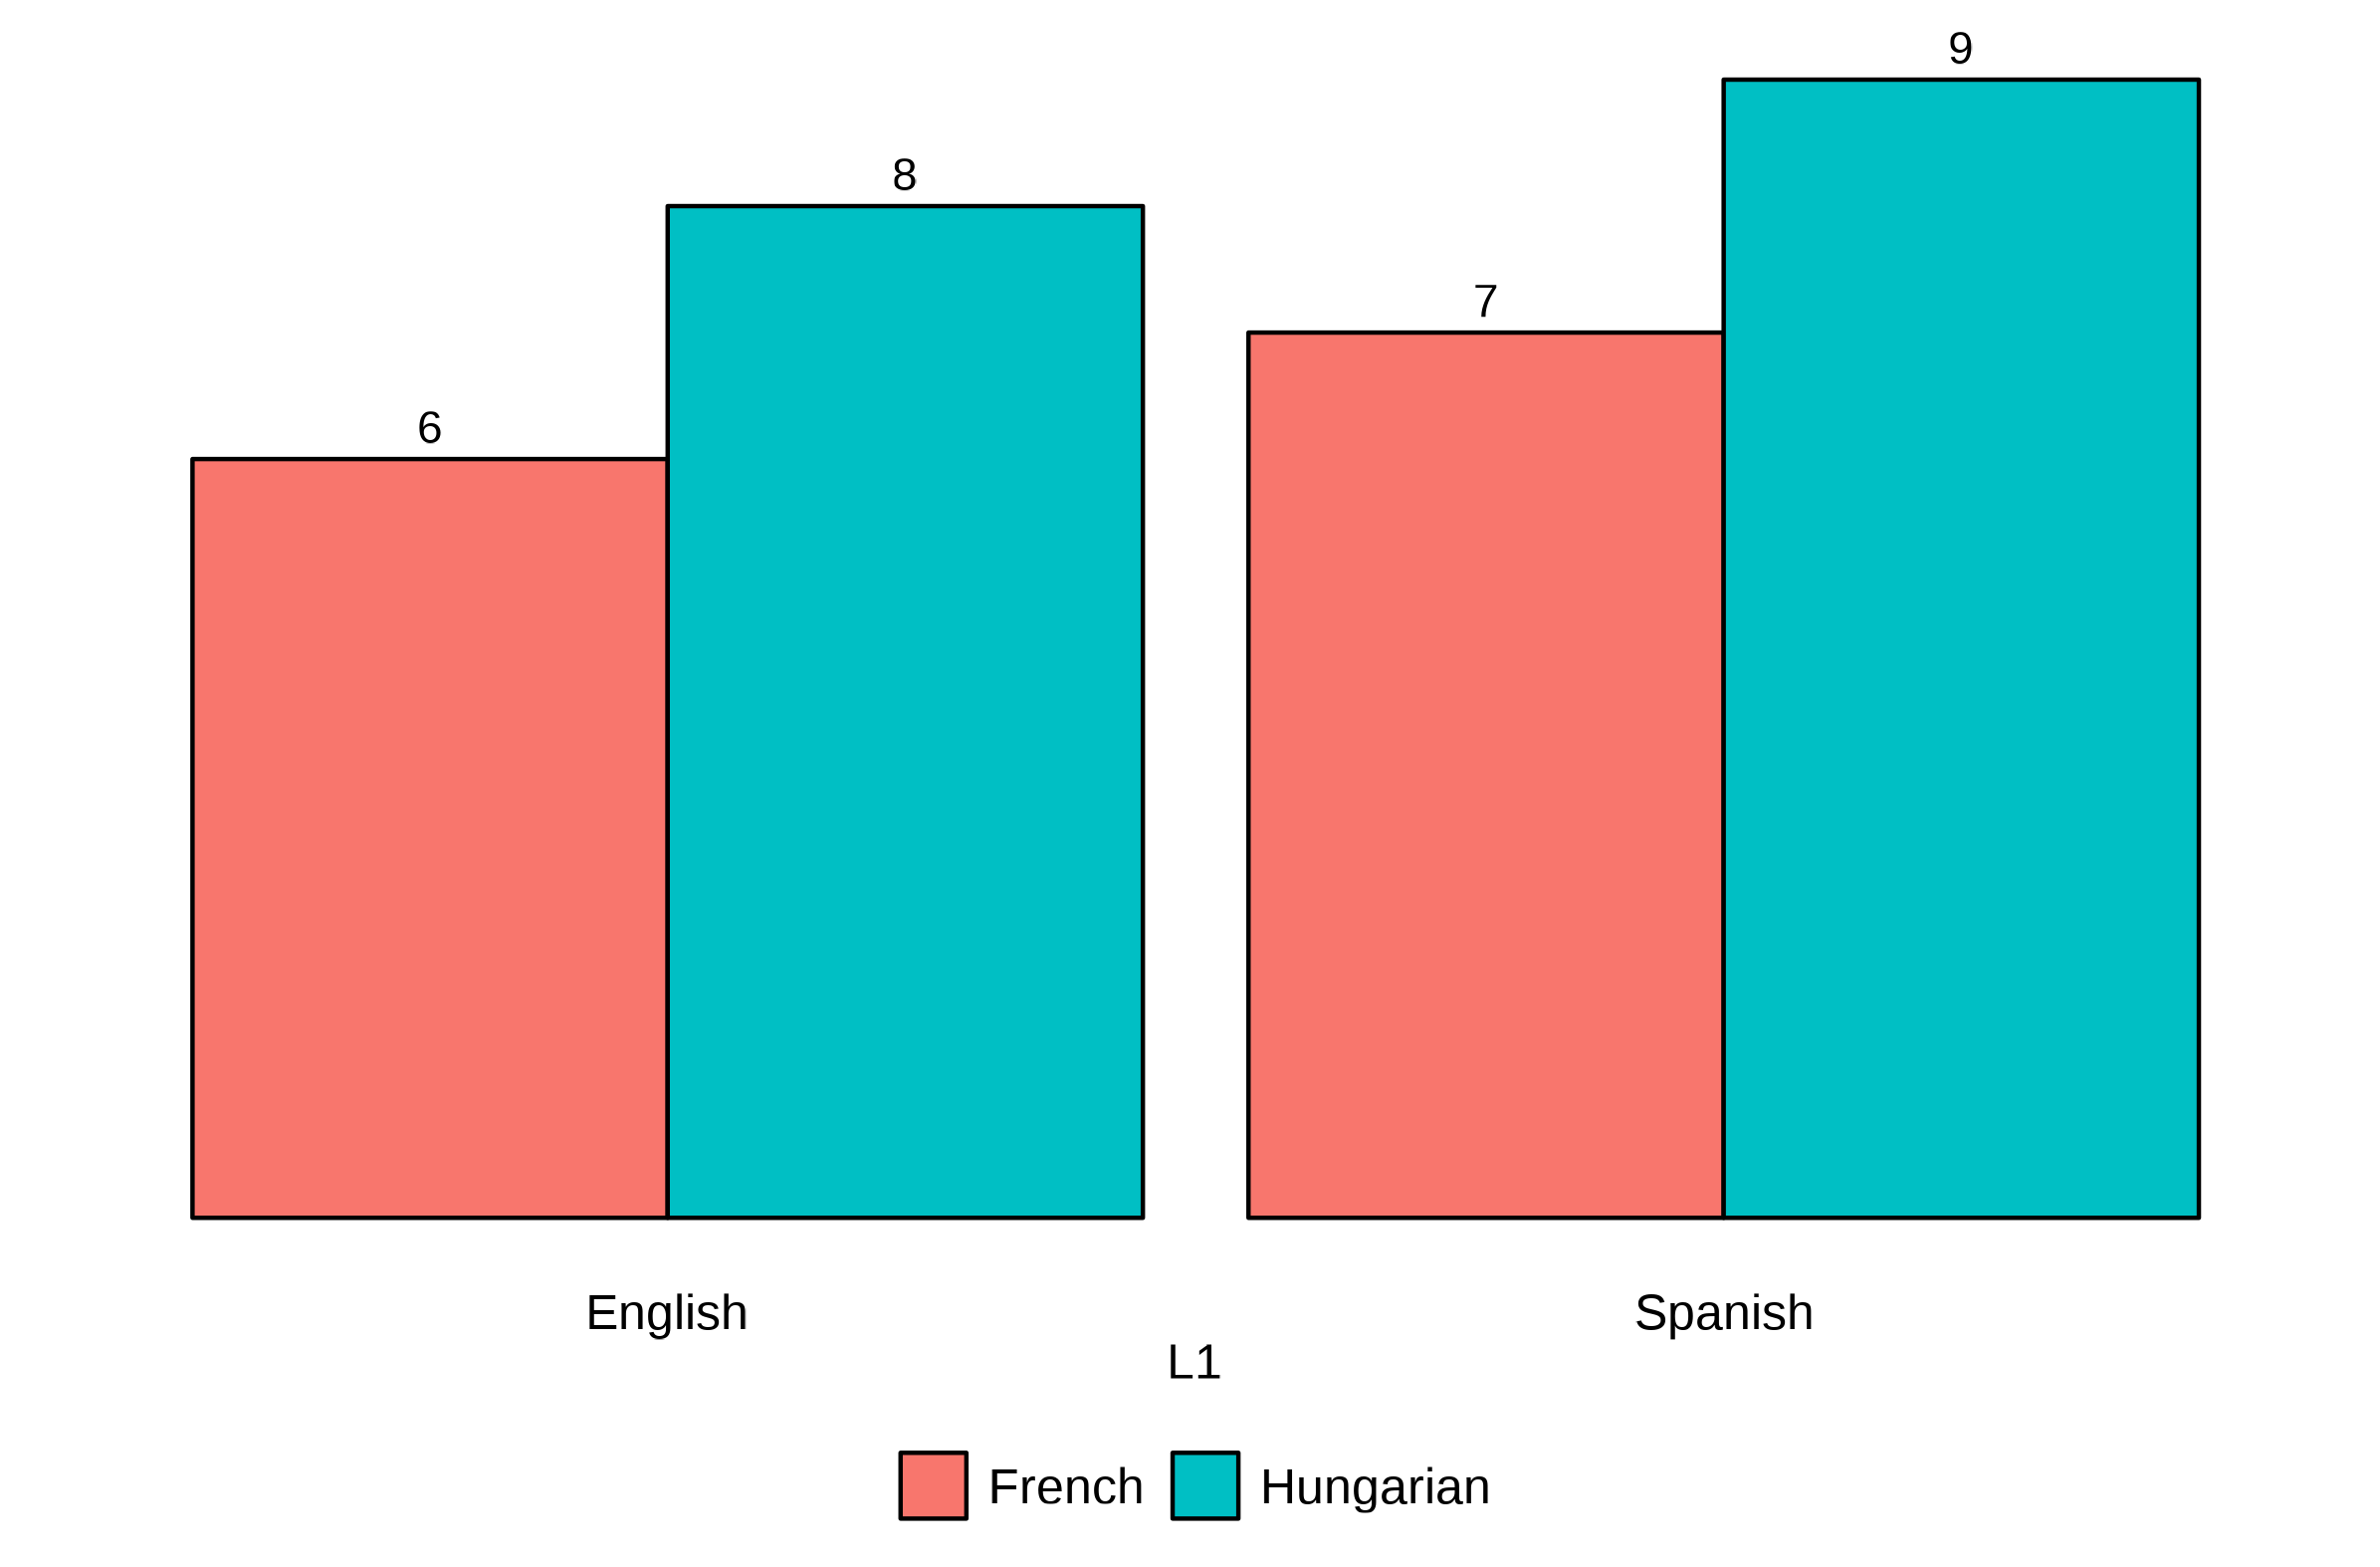
\includegraphics[width=425px]{new_docs/img/dpbe_ppts} \caption{ }\label{fig:unnamed-chunk-2}
\end{figure}

\textbf{Group-level S-shaped curve for all 30 DPBE ppts}

\begin{figure}
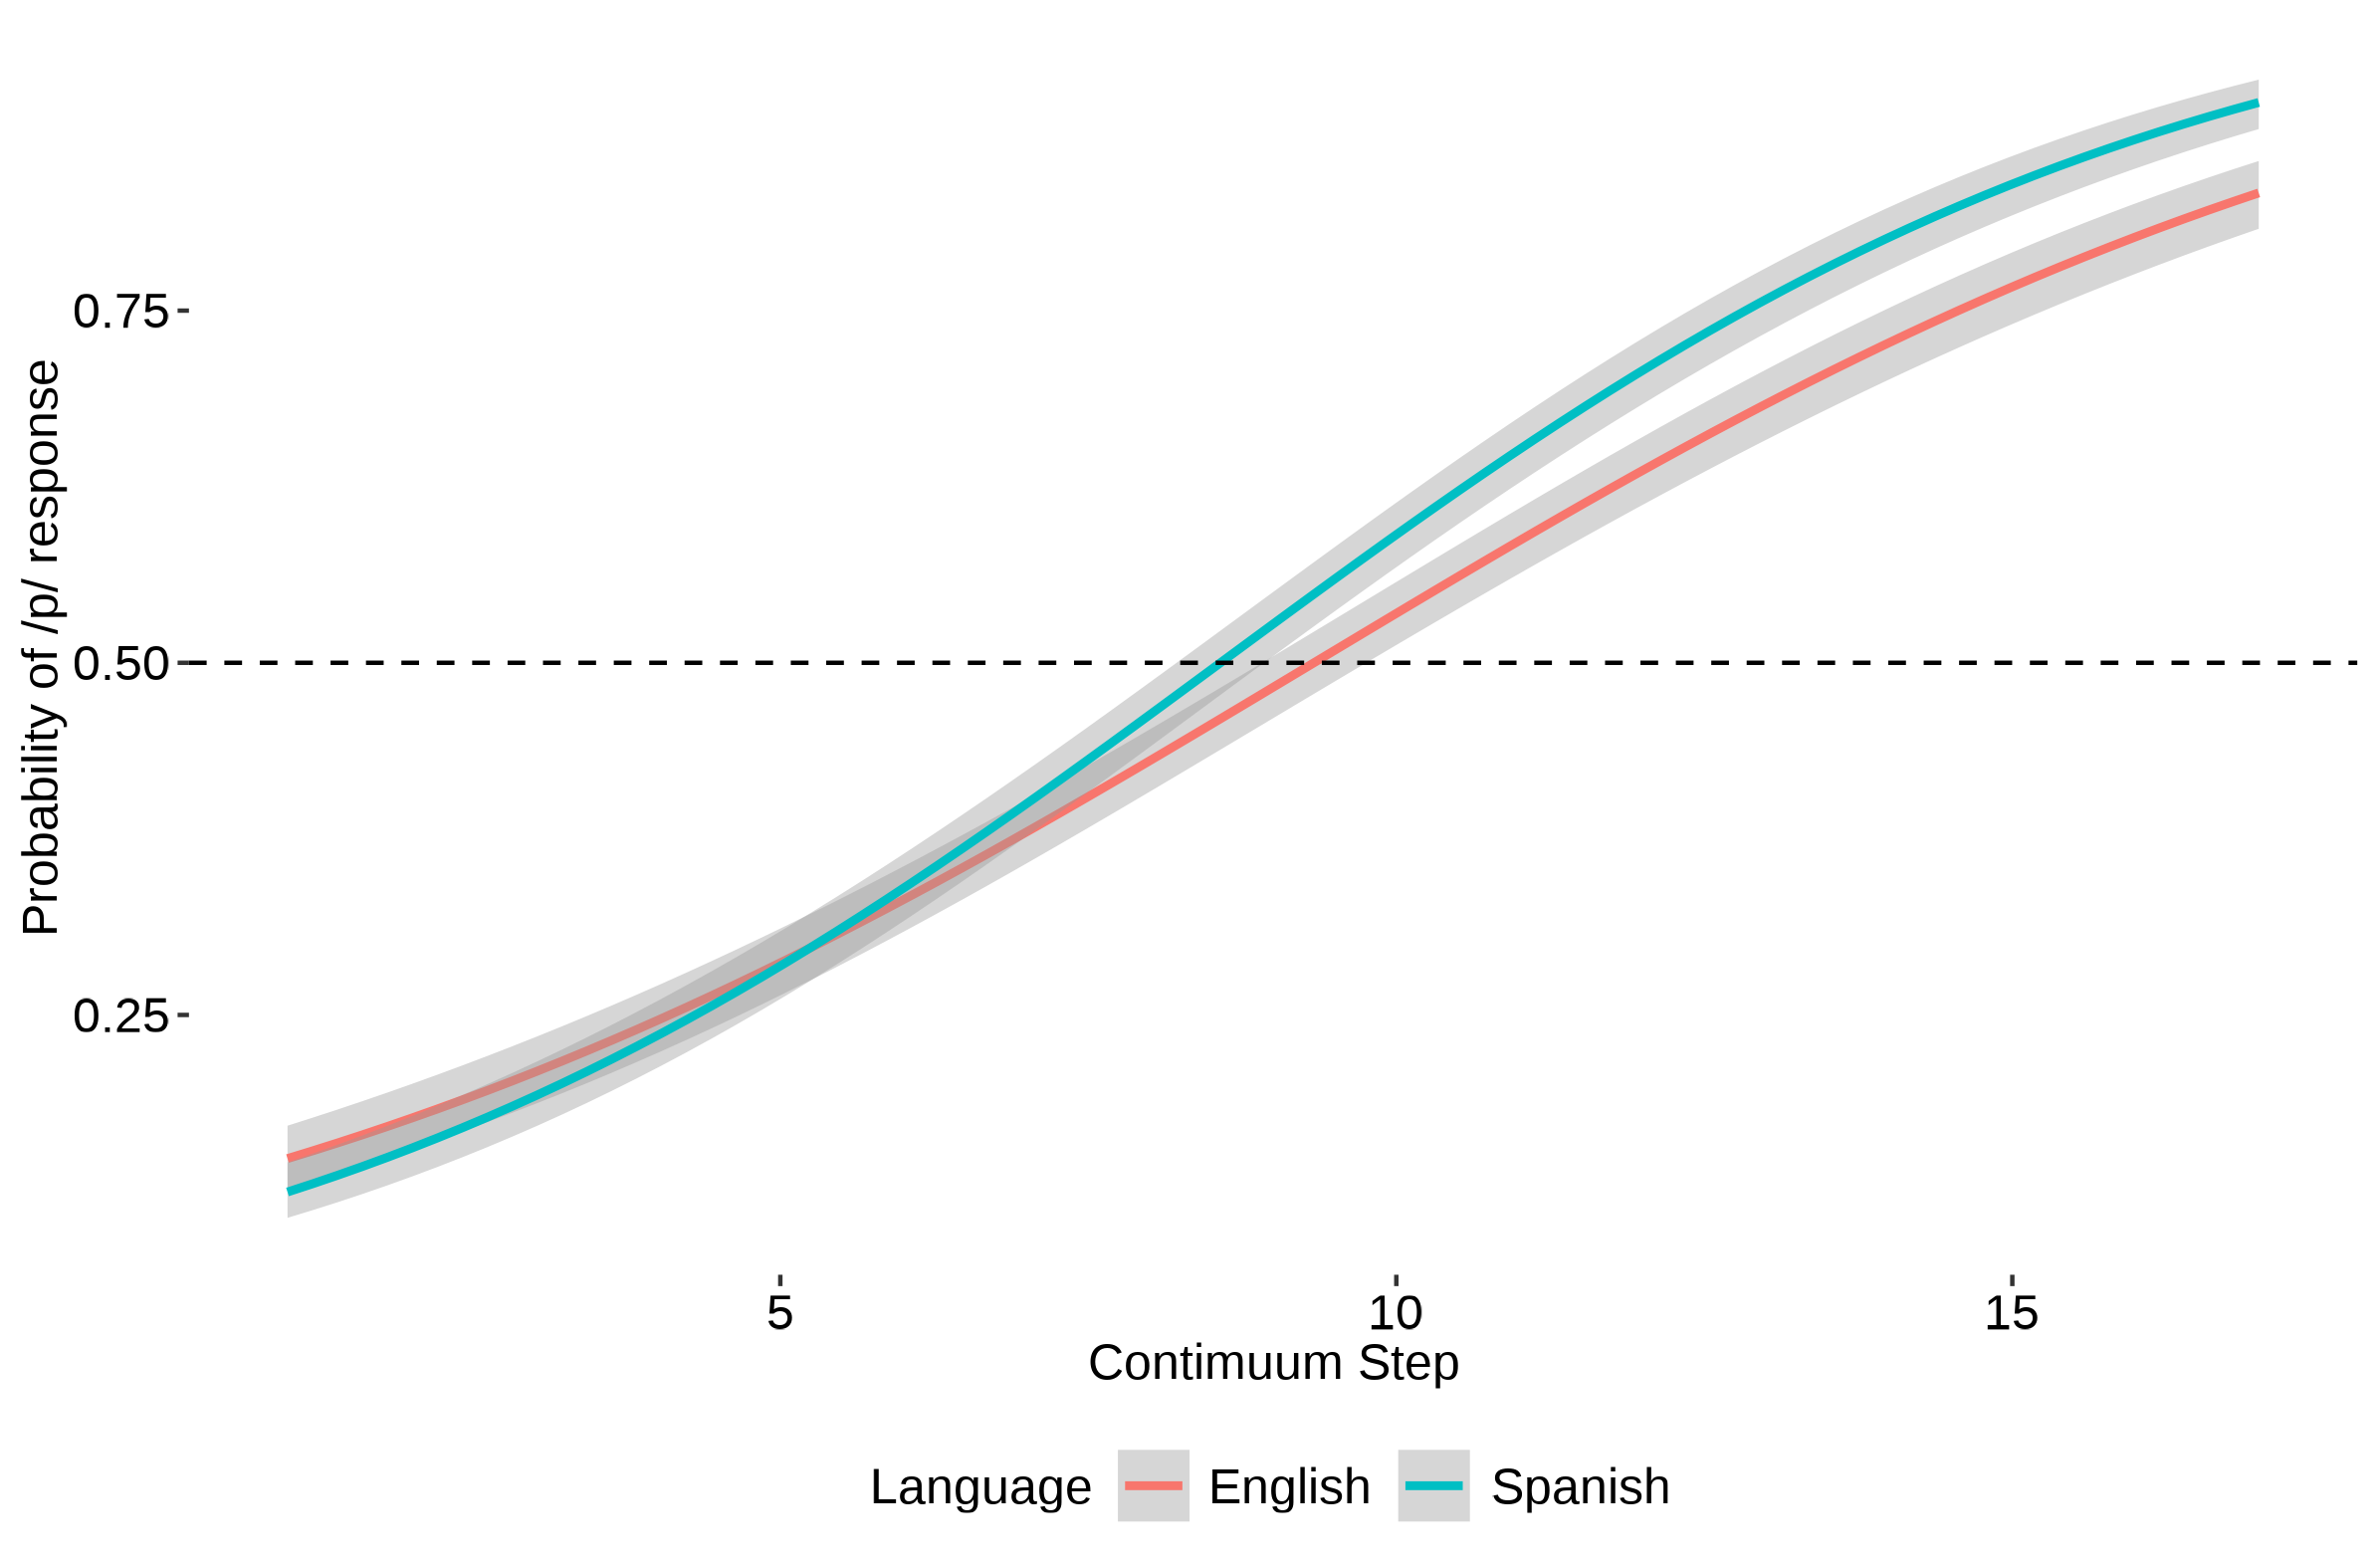
\includegraphics[width=425px]{new_docs/img/dpbe_ppts_s} \caption{ }\label{fig:unnamed-chunk-3}
\end{figure}

\textbf{Group-level S-shaped curve for all 31 non-DPBE ppts}

\begin{figure}
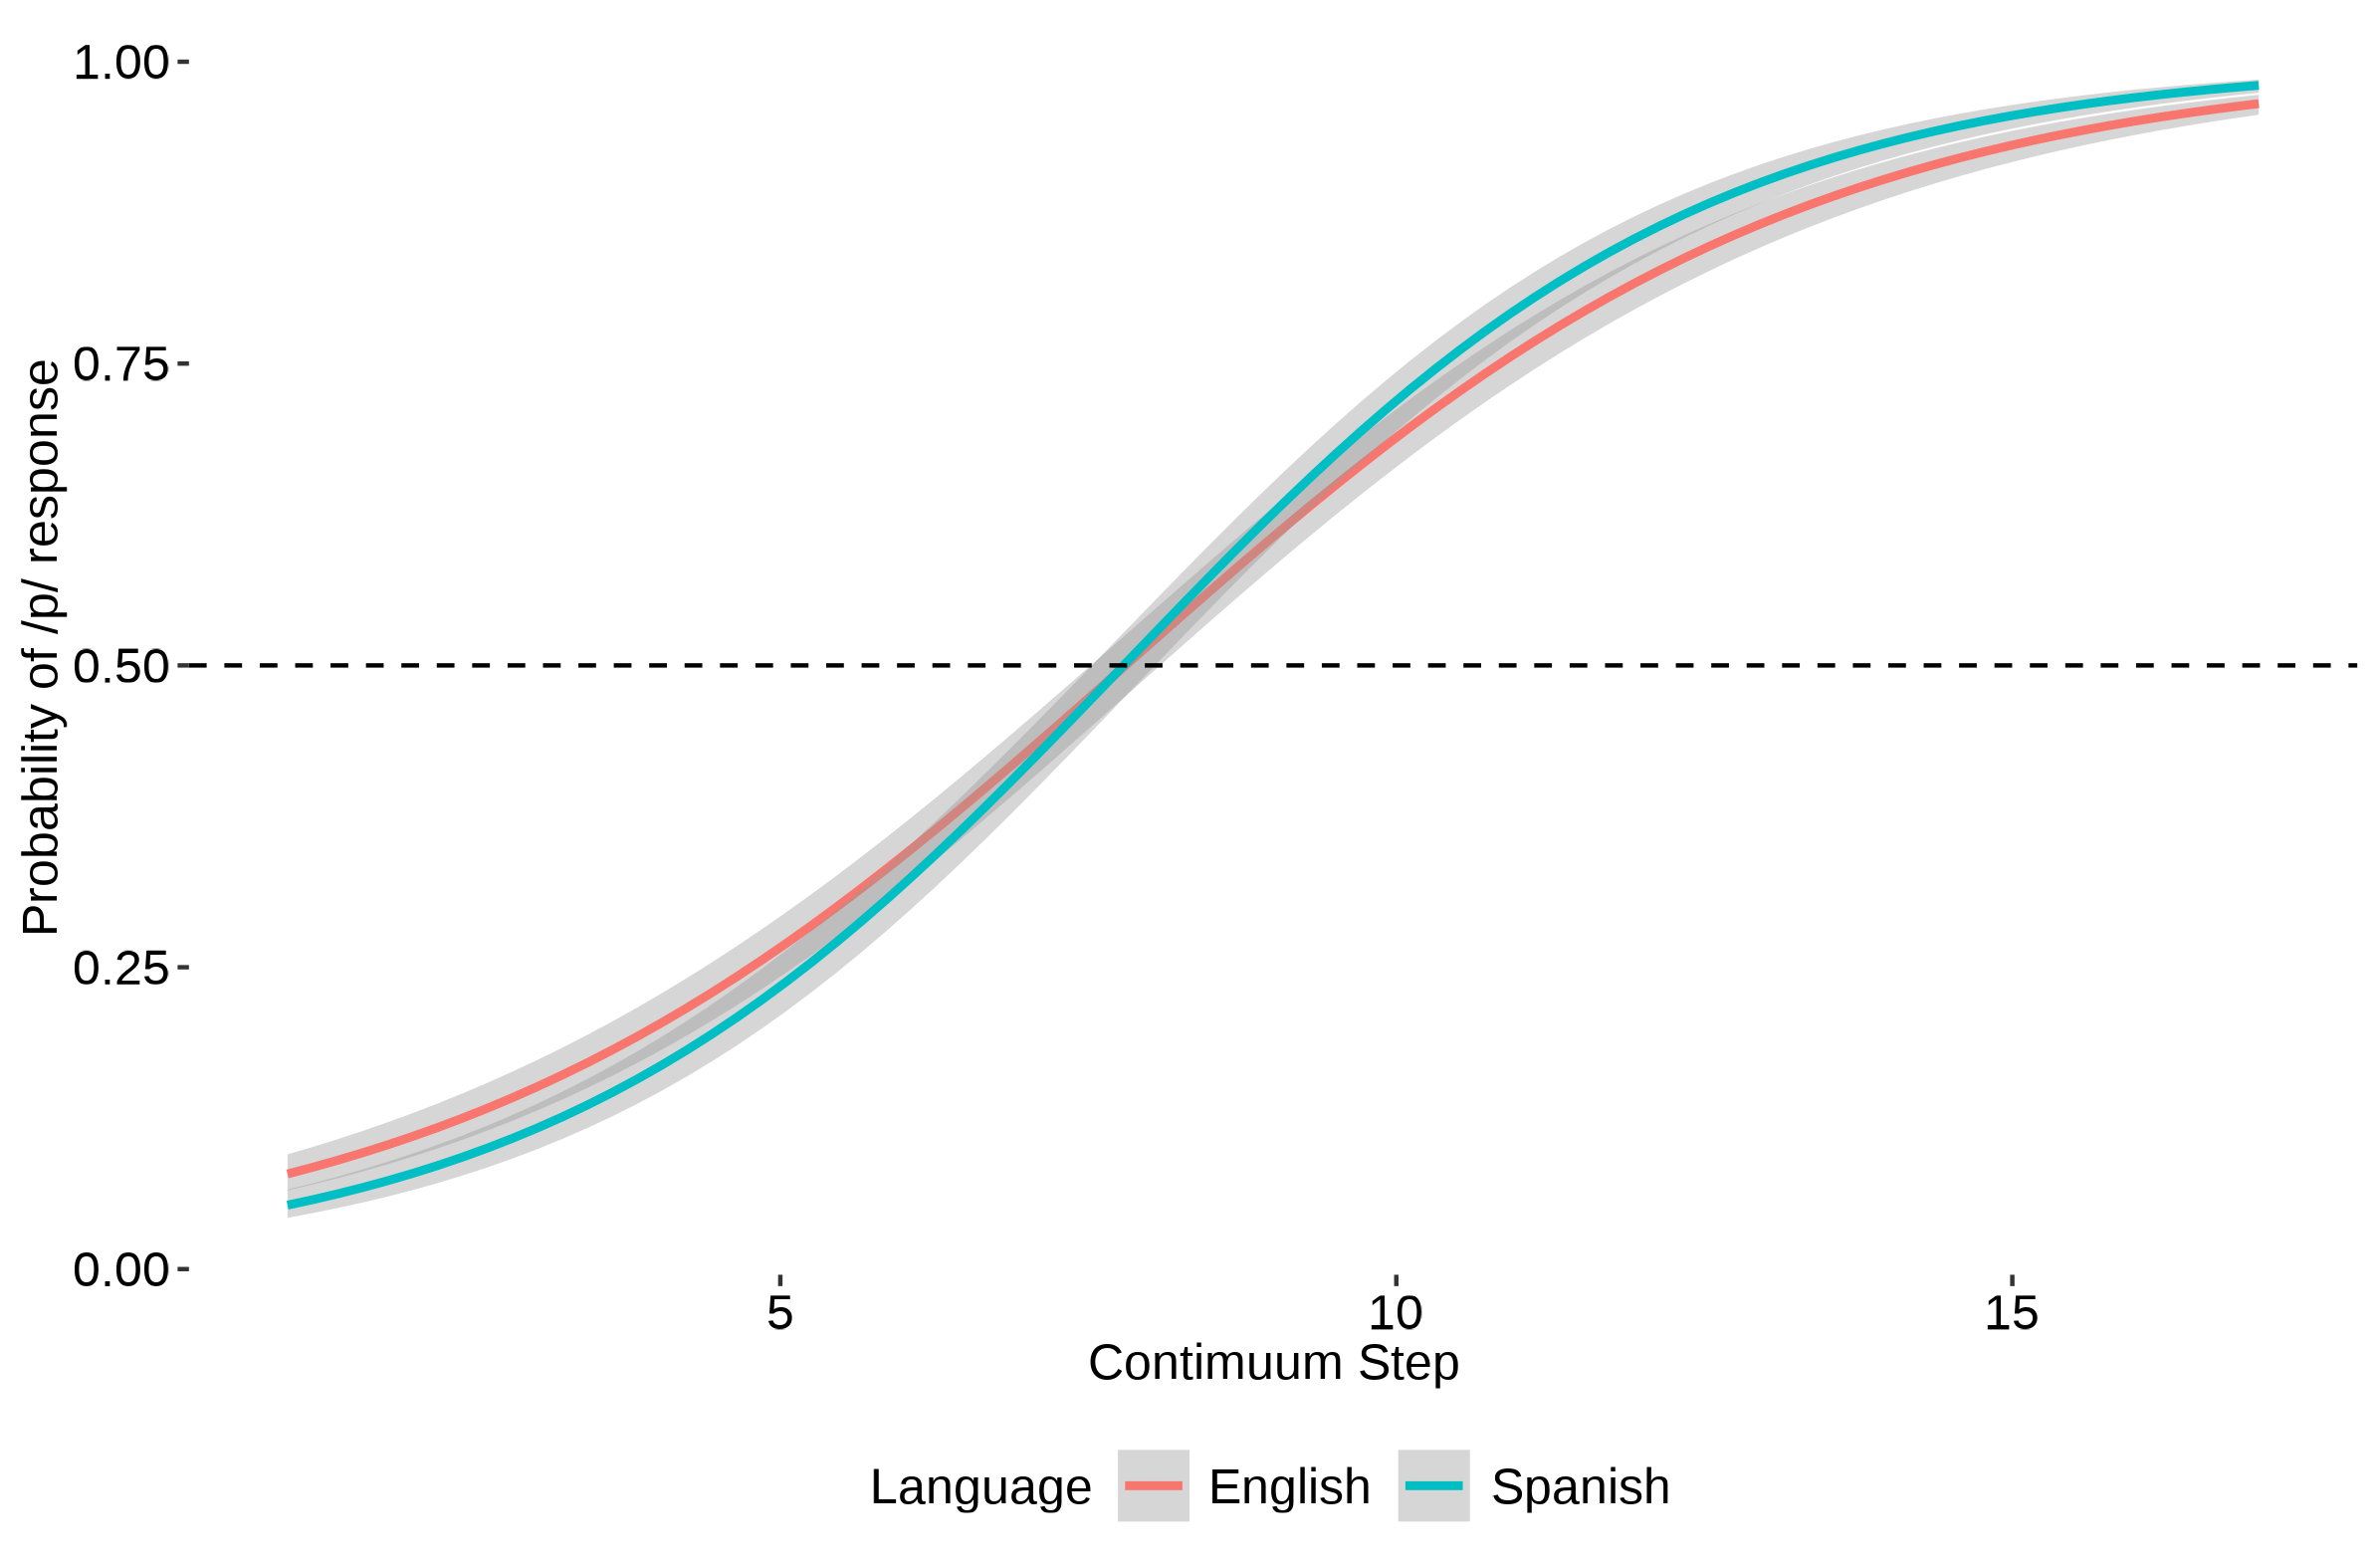
\includegraphics[width=425px]{new_docs/img/dpbe_no_ppts_s} \caption{ }\label{fig:unnamed-chunk-4}
\end{figure}

\textbf{Breakdown of L1 and ``L3'' for participants with a Spanish-like L3}

\begin{figure}
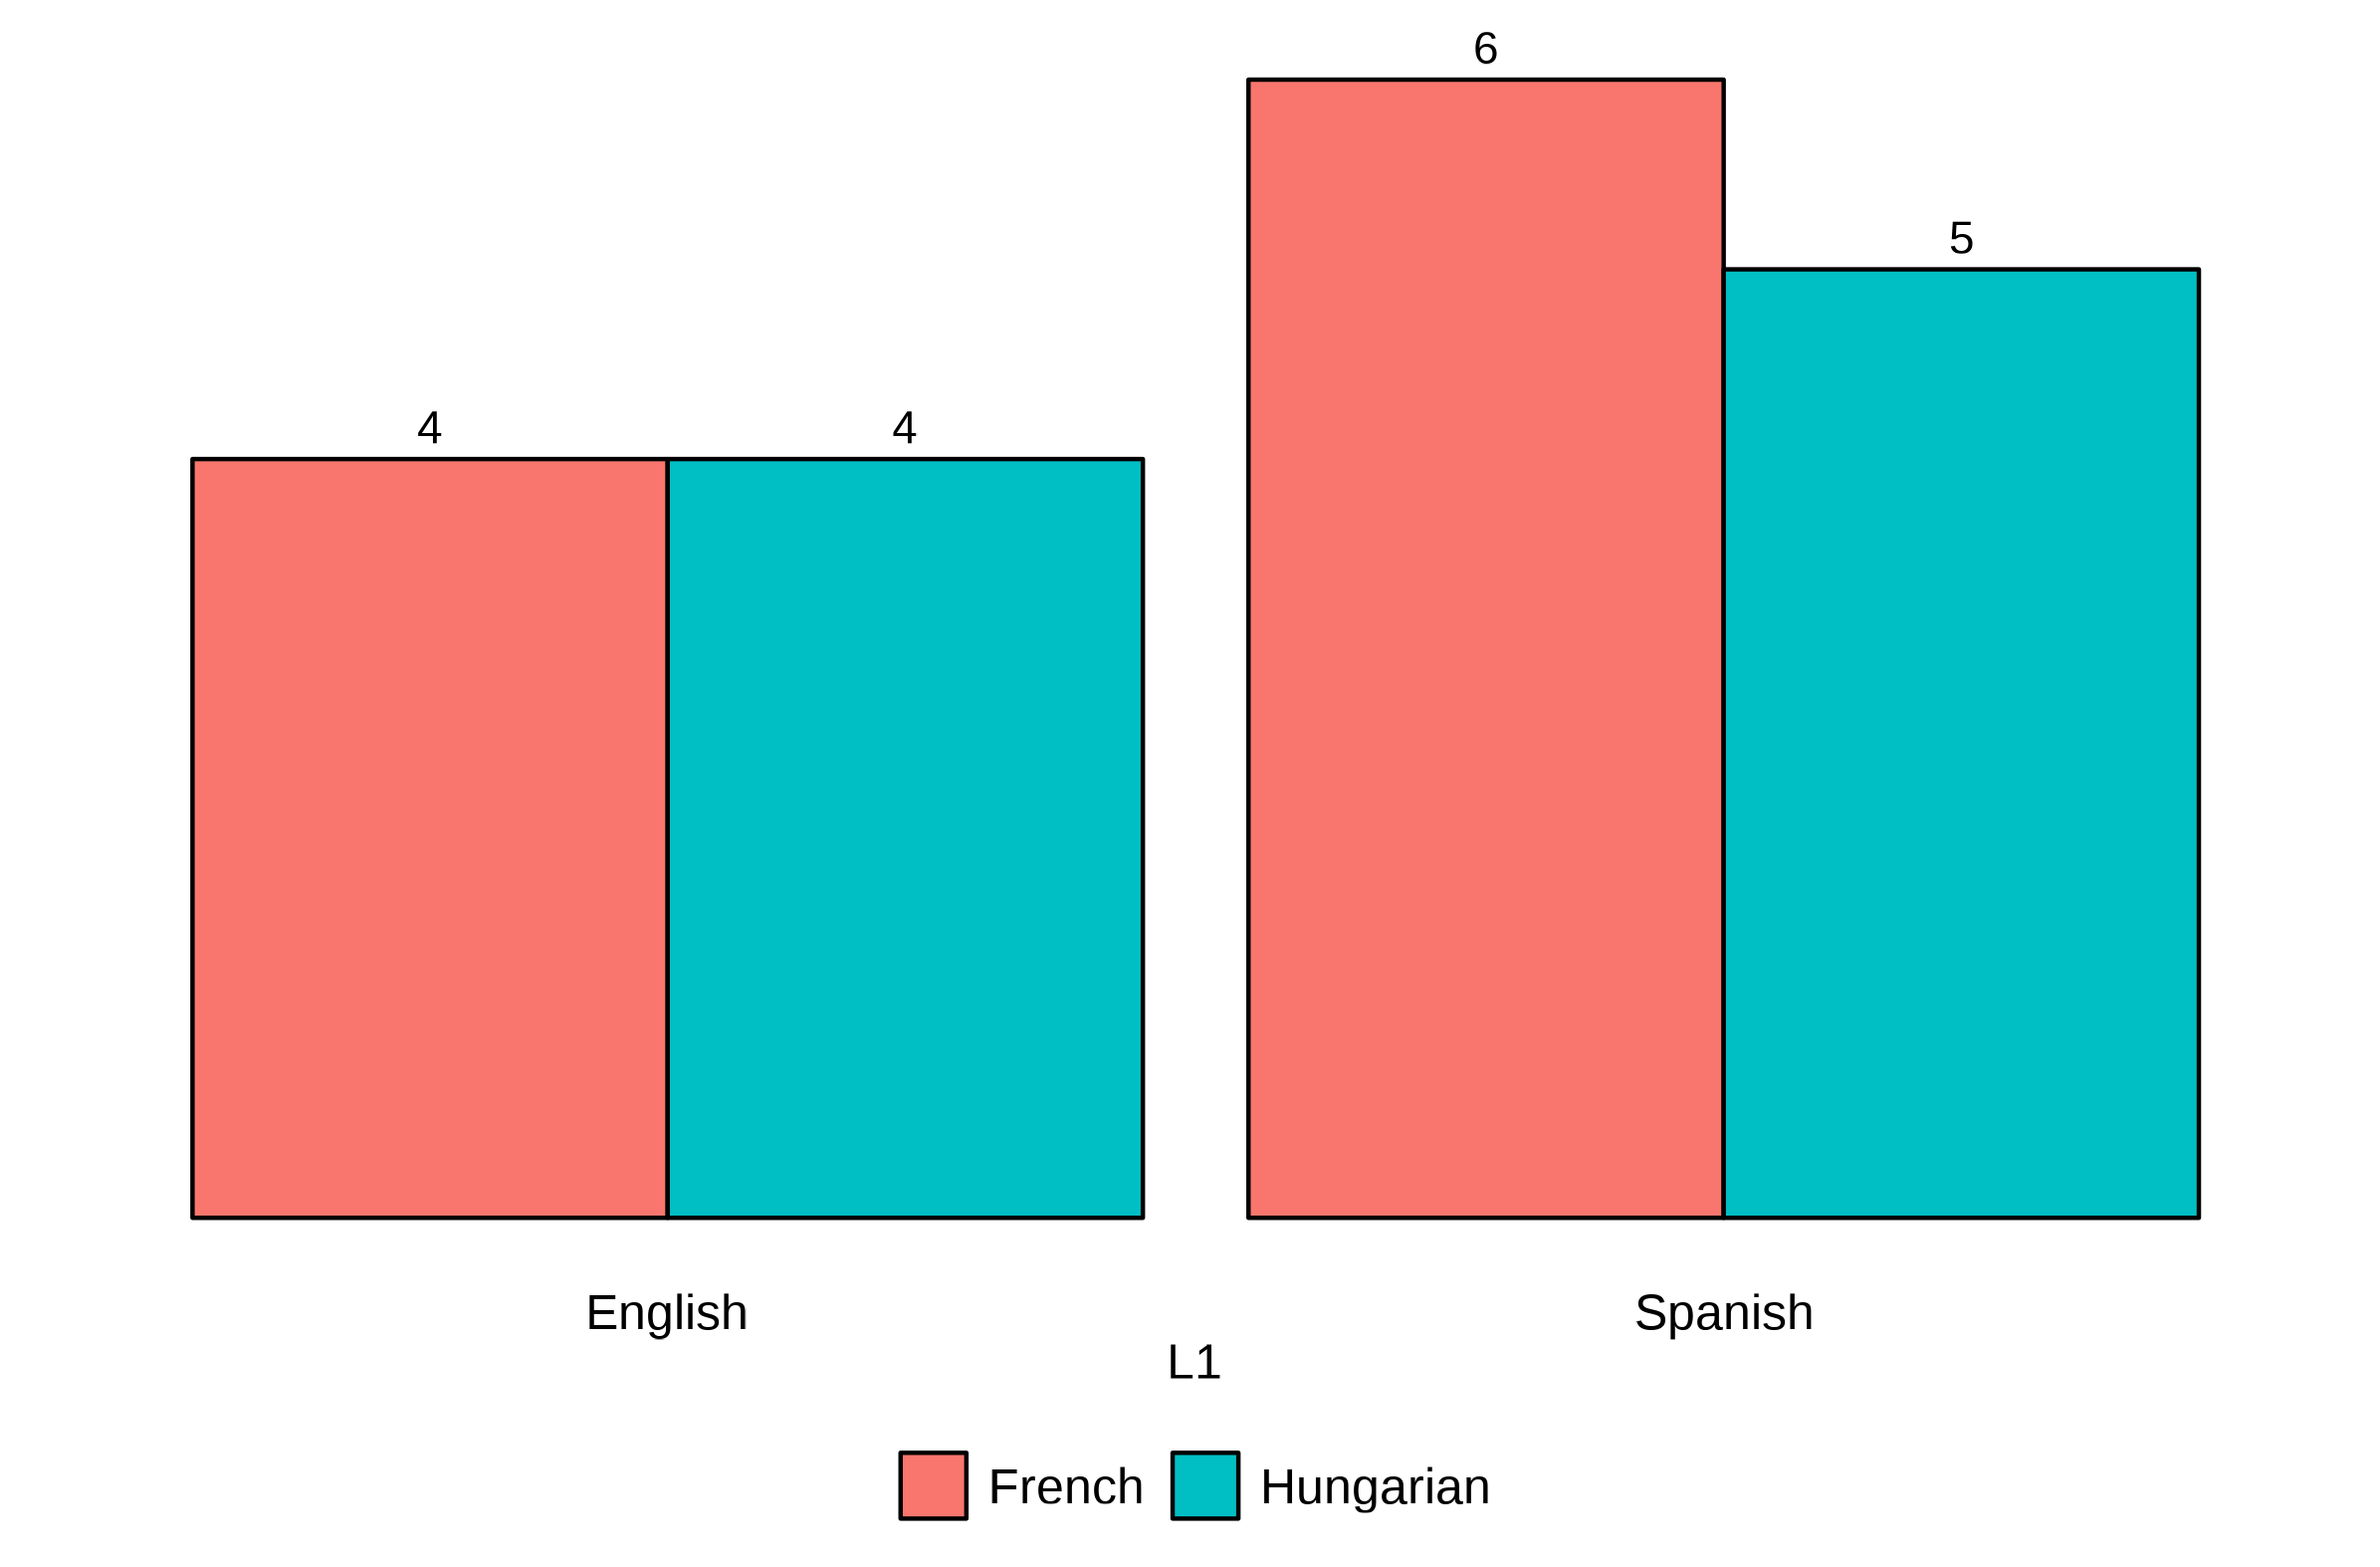
\includegraphics[width=425px]{new_docs/img/dpbe_span_ppts} \caption{ }\label{fig:unnamed-chunk-5}
\end{figure}

\textbf{Group-level S-shaped curve for all Spanish-like boundaries}

\begin{figure}
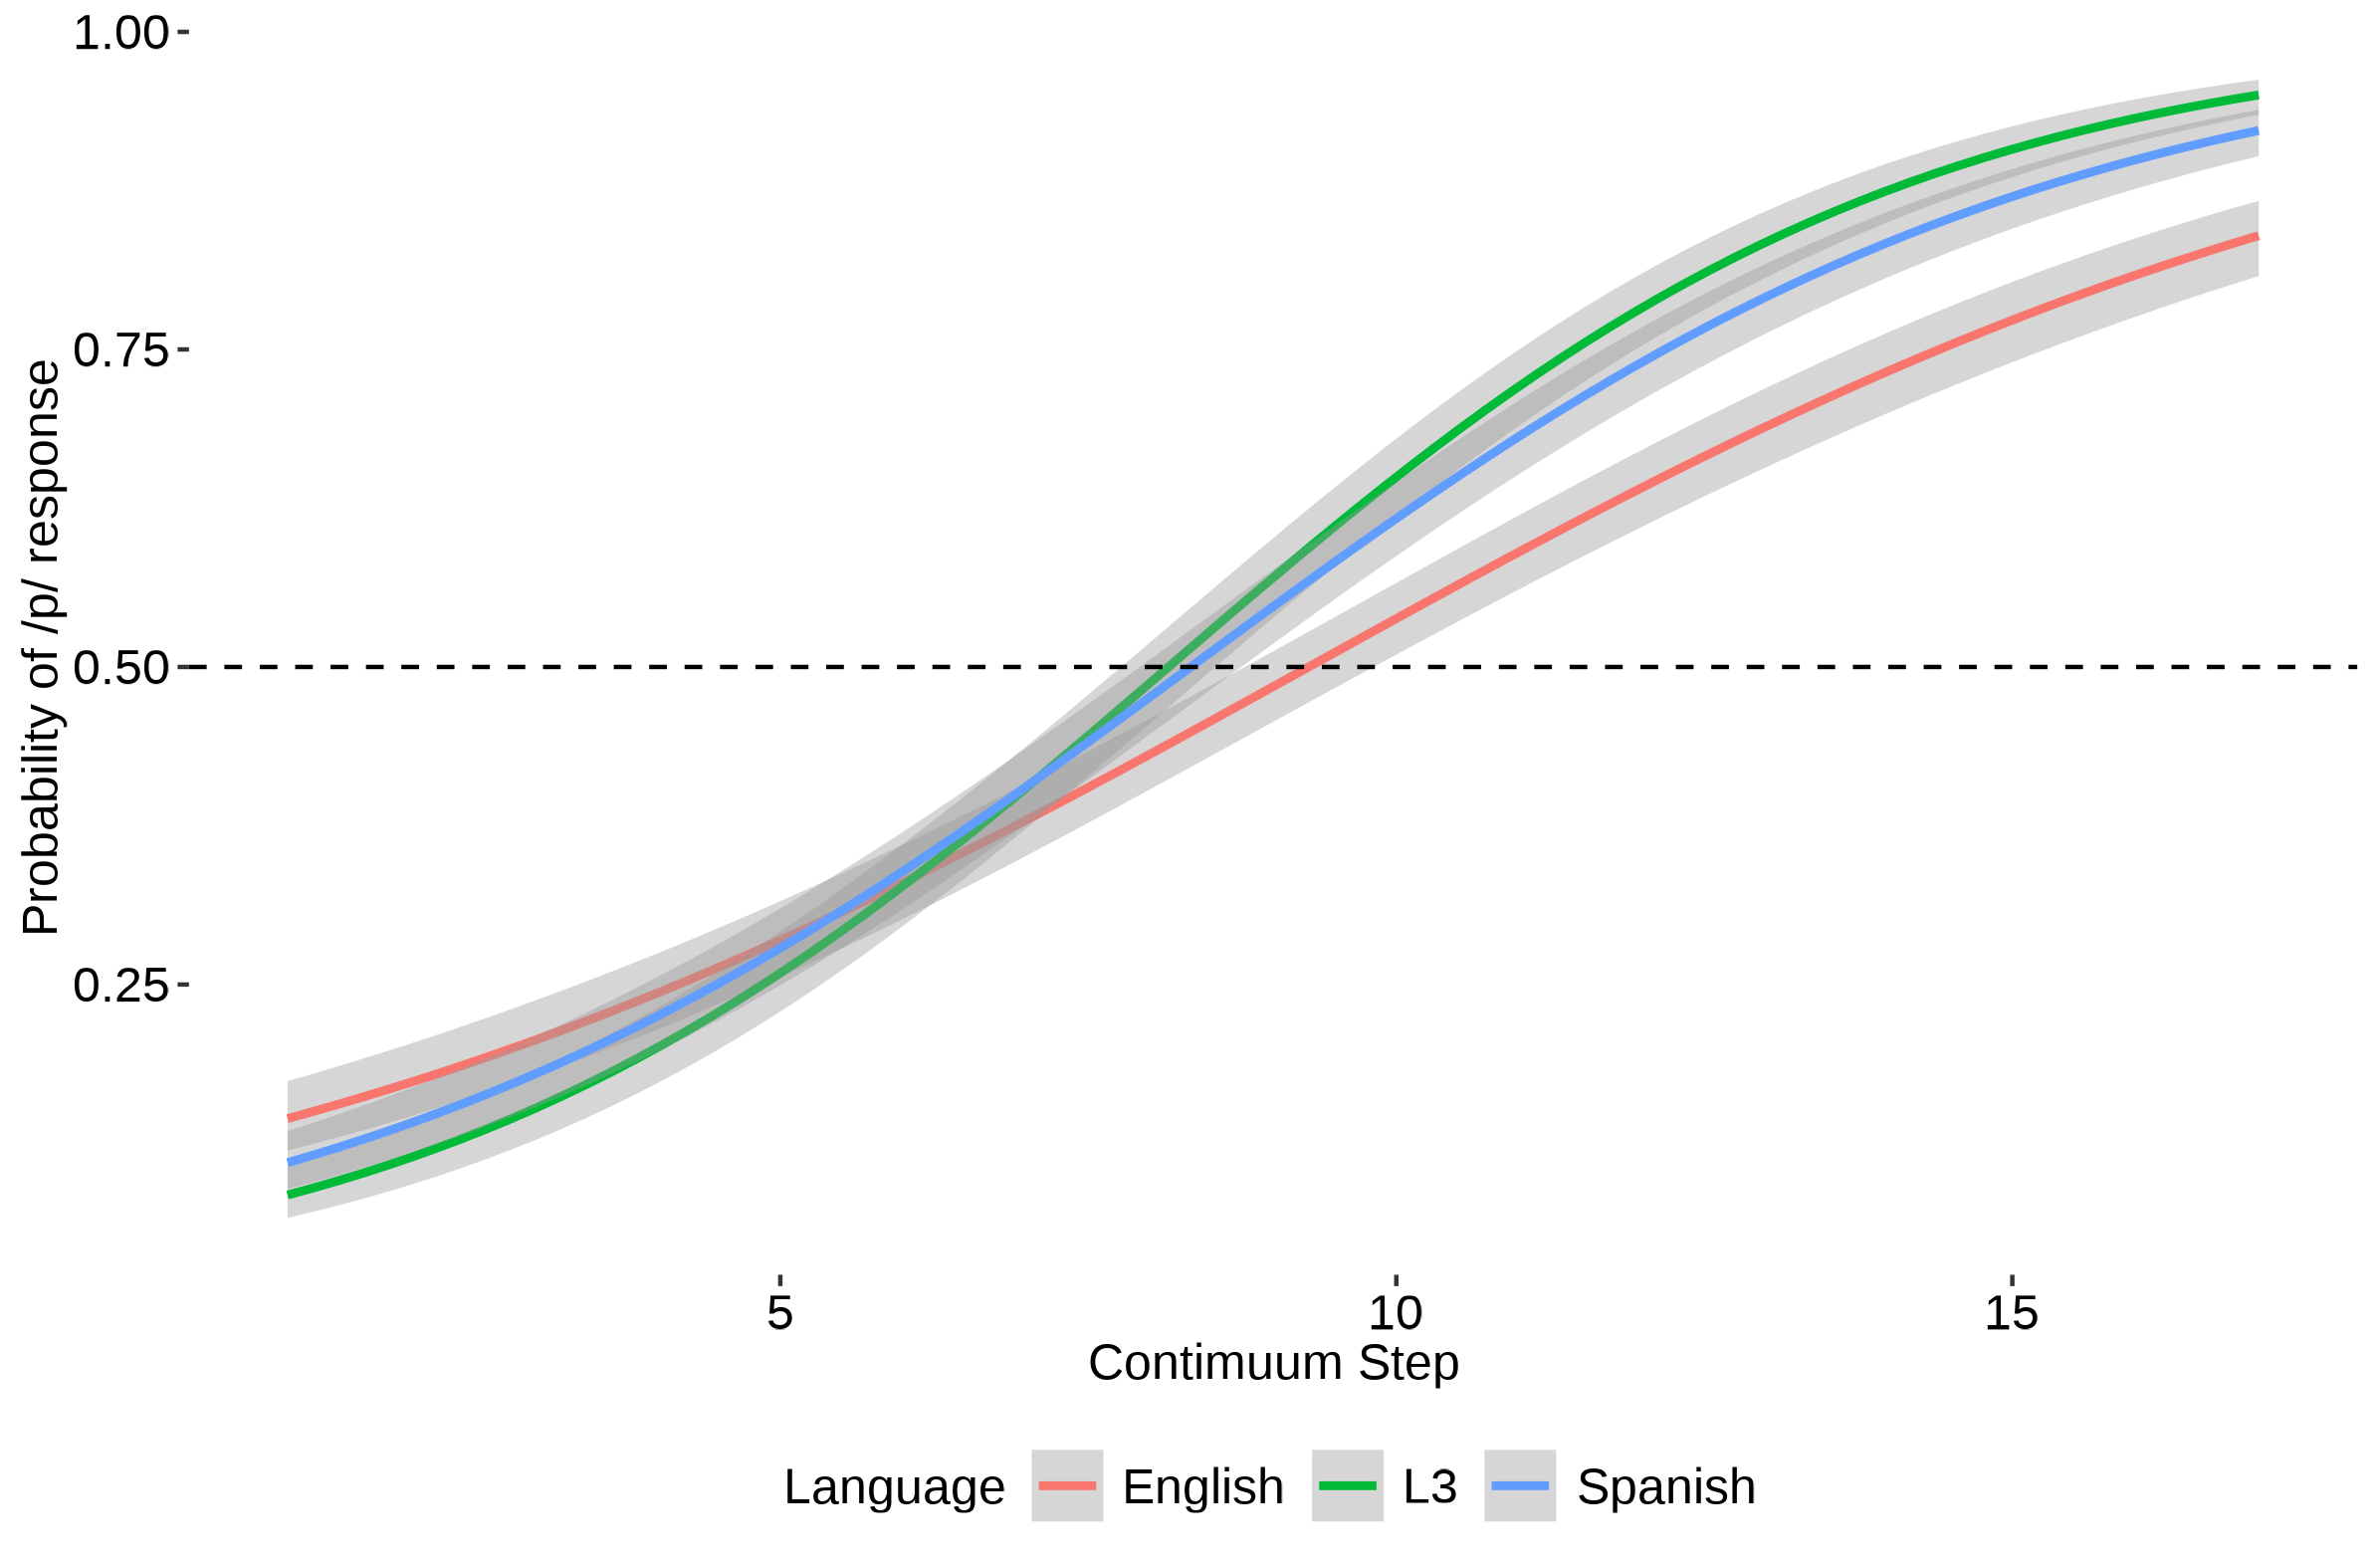
\includegraphics[width=425px]{new_docs/img/dpbe_ppts_sb} \caption{ }\label{fig:unnamed-chunk-6}
\end{figure}

\textbf{Breakdown of L1 and ``L3'' for participants with a English-like L3}

\begin{figure}
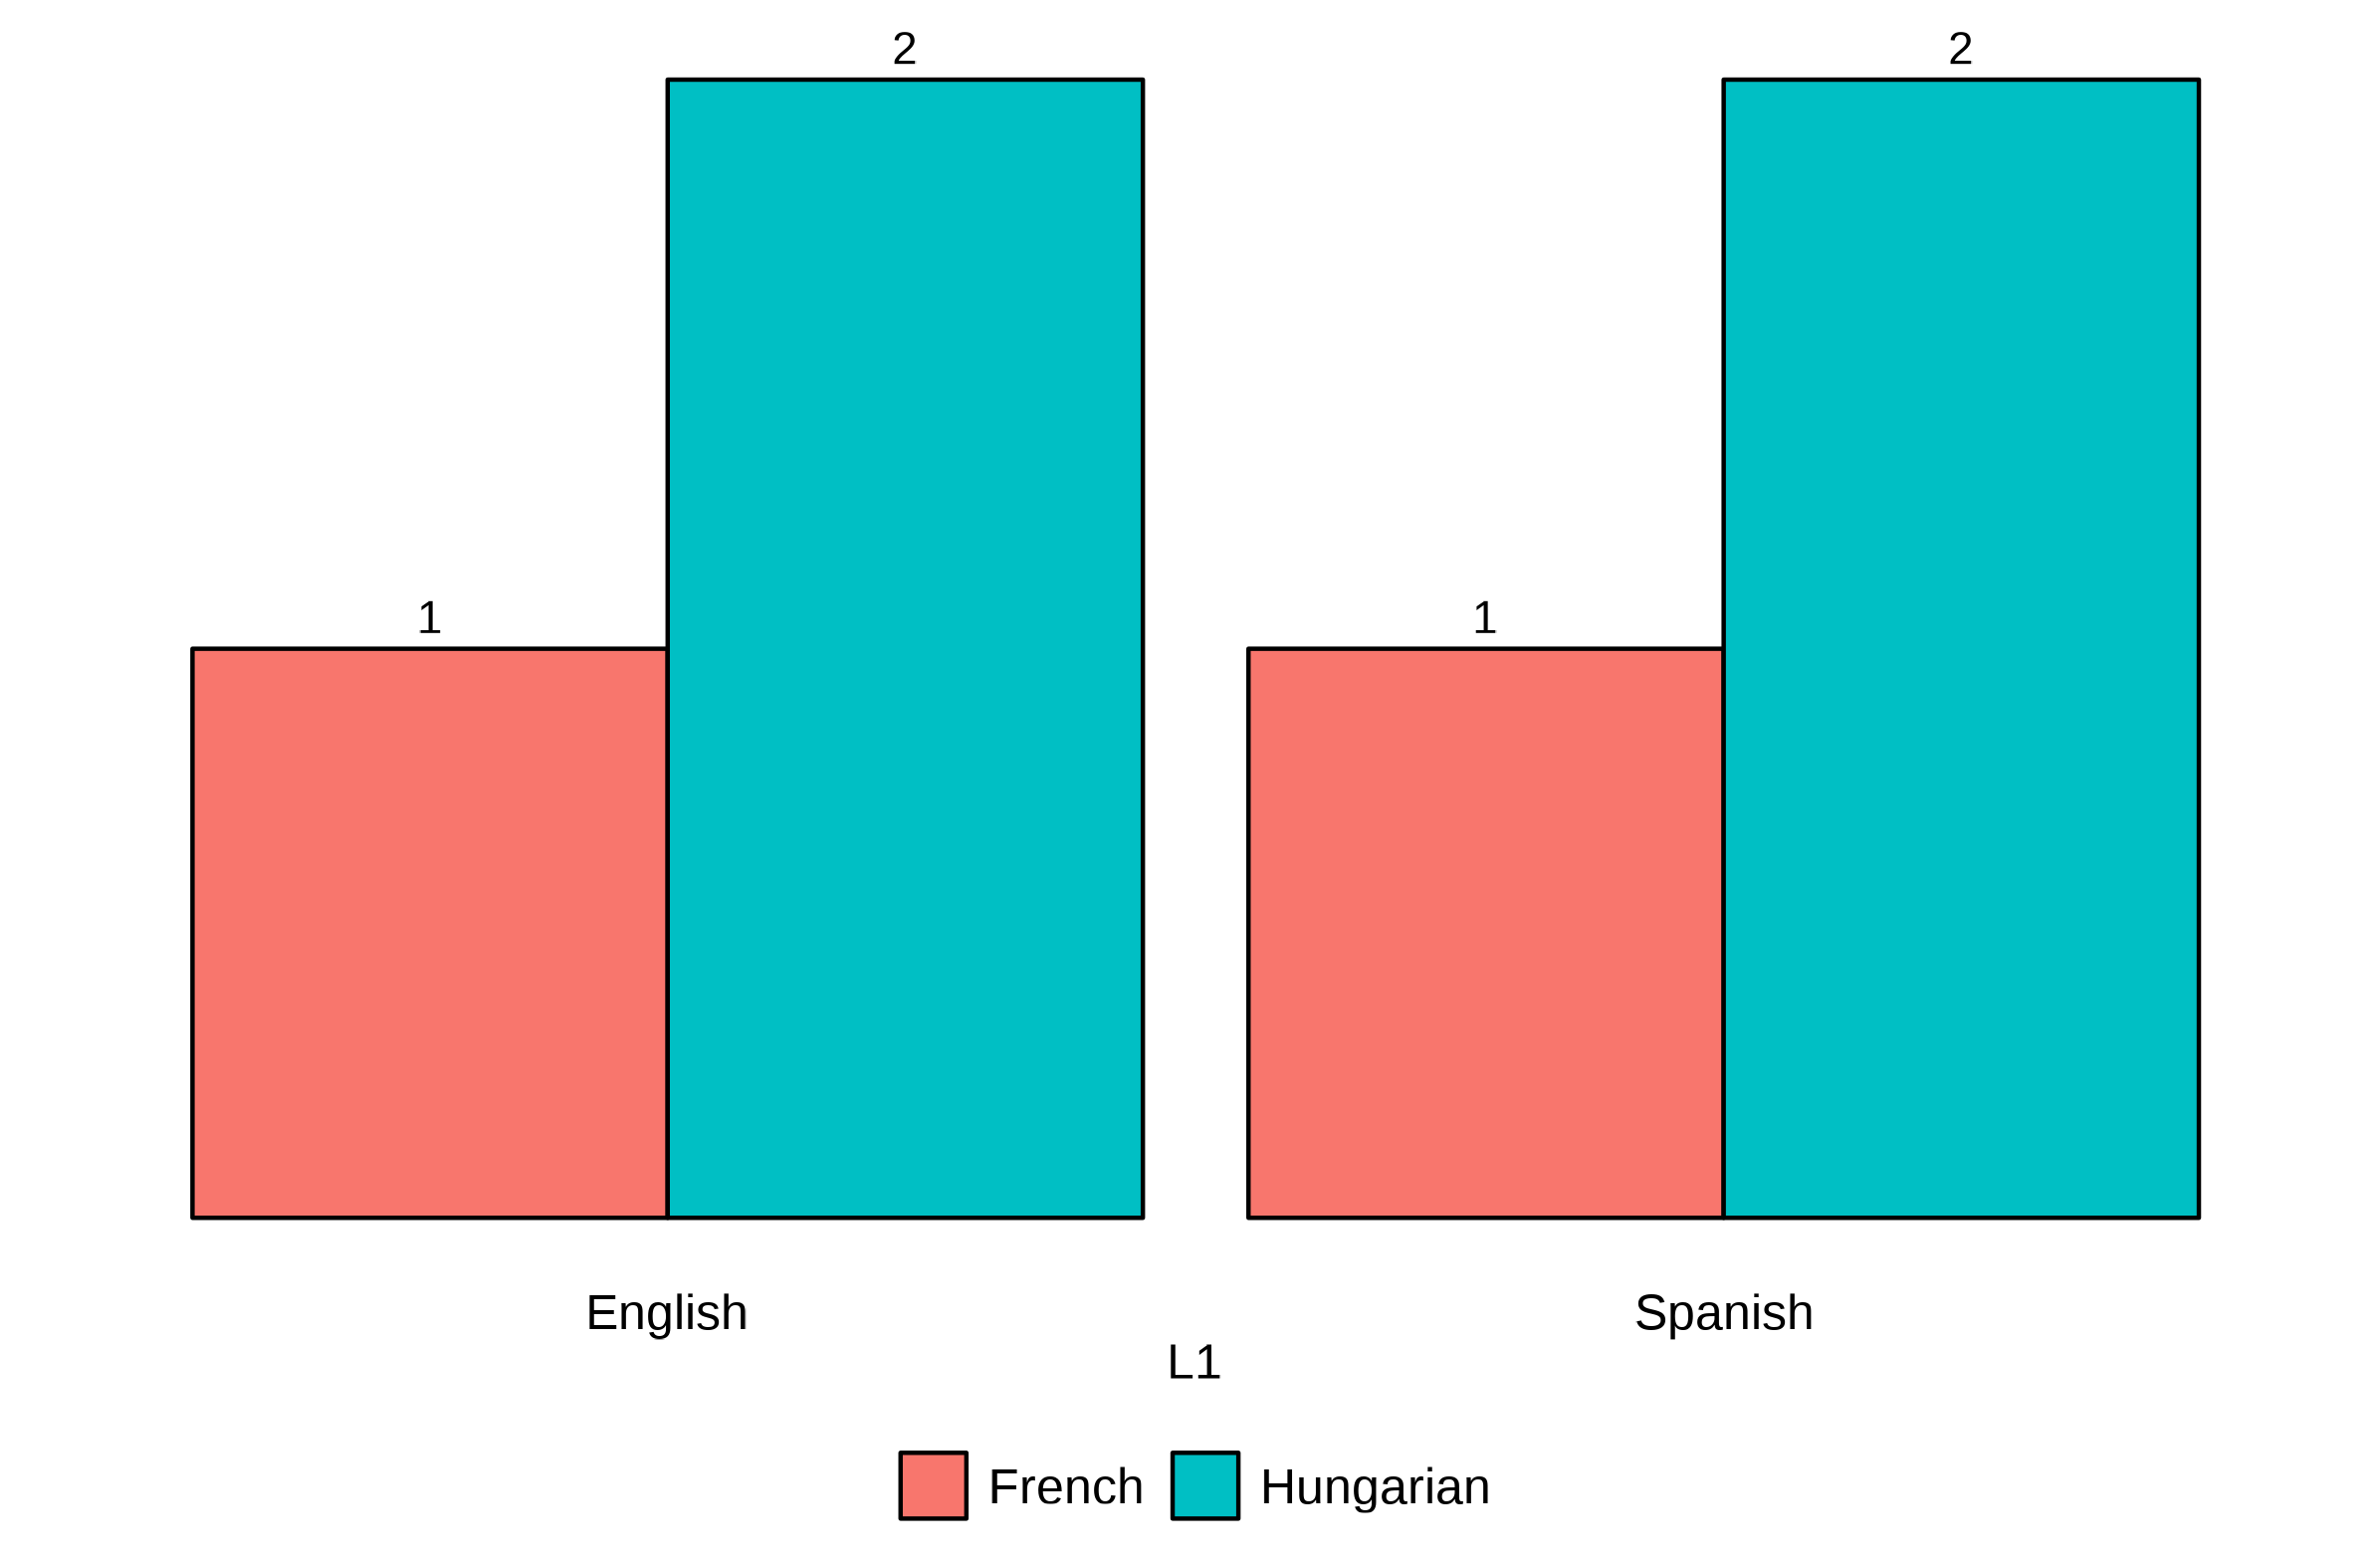
\includegraphics[width=425px]{new_docs/img/dpbe_eng_ppts} \caption{ }\label{fig:unnamed-chunk-7}
\end{figure}

\textbf{Group-level S-shaped curve for all English-like boundaries}

\begin{figure}
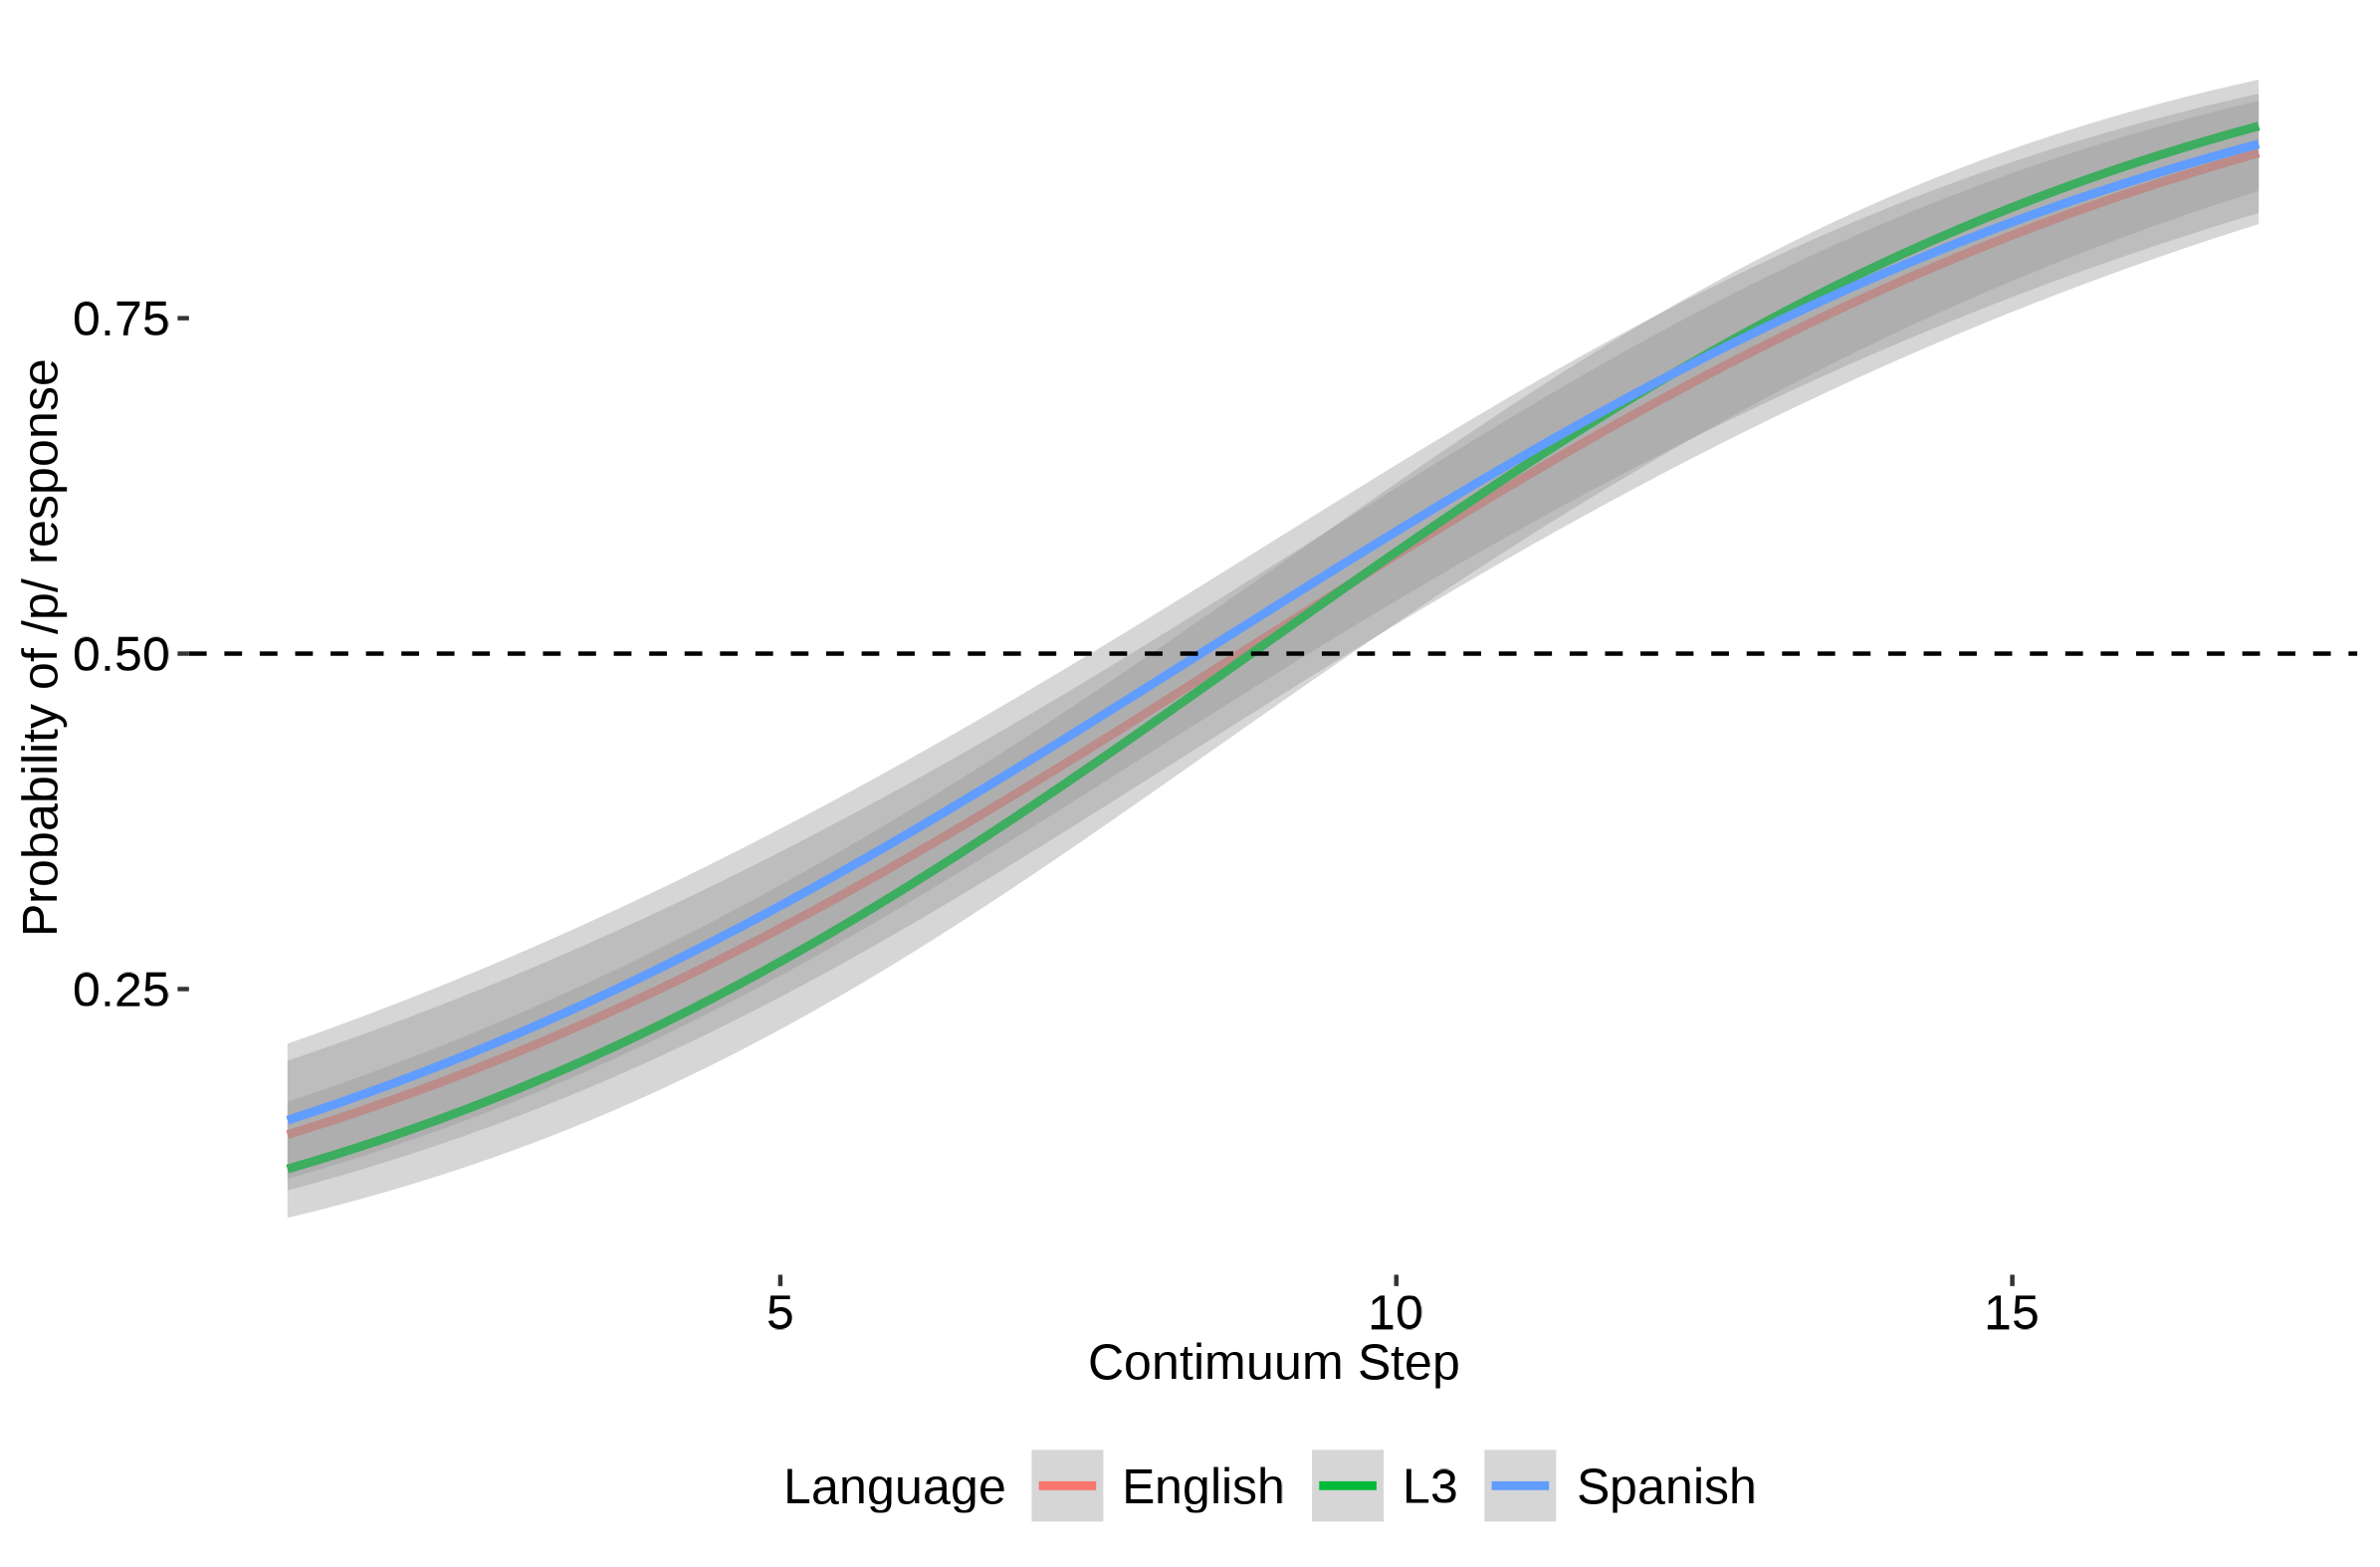
\includegraphics[width=425px]{new_docs/img/dpbe_ppts_eng} \caption{ }\label{fig:unnamed-chunk-8}
\end{figure}

\begin{figure}
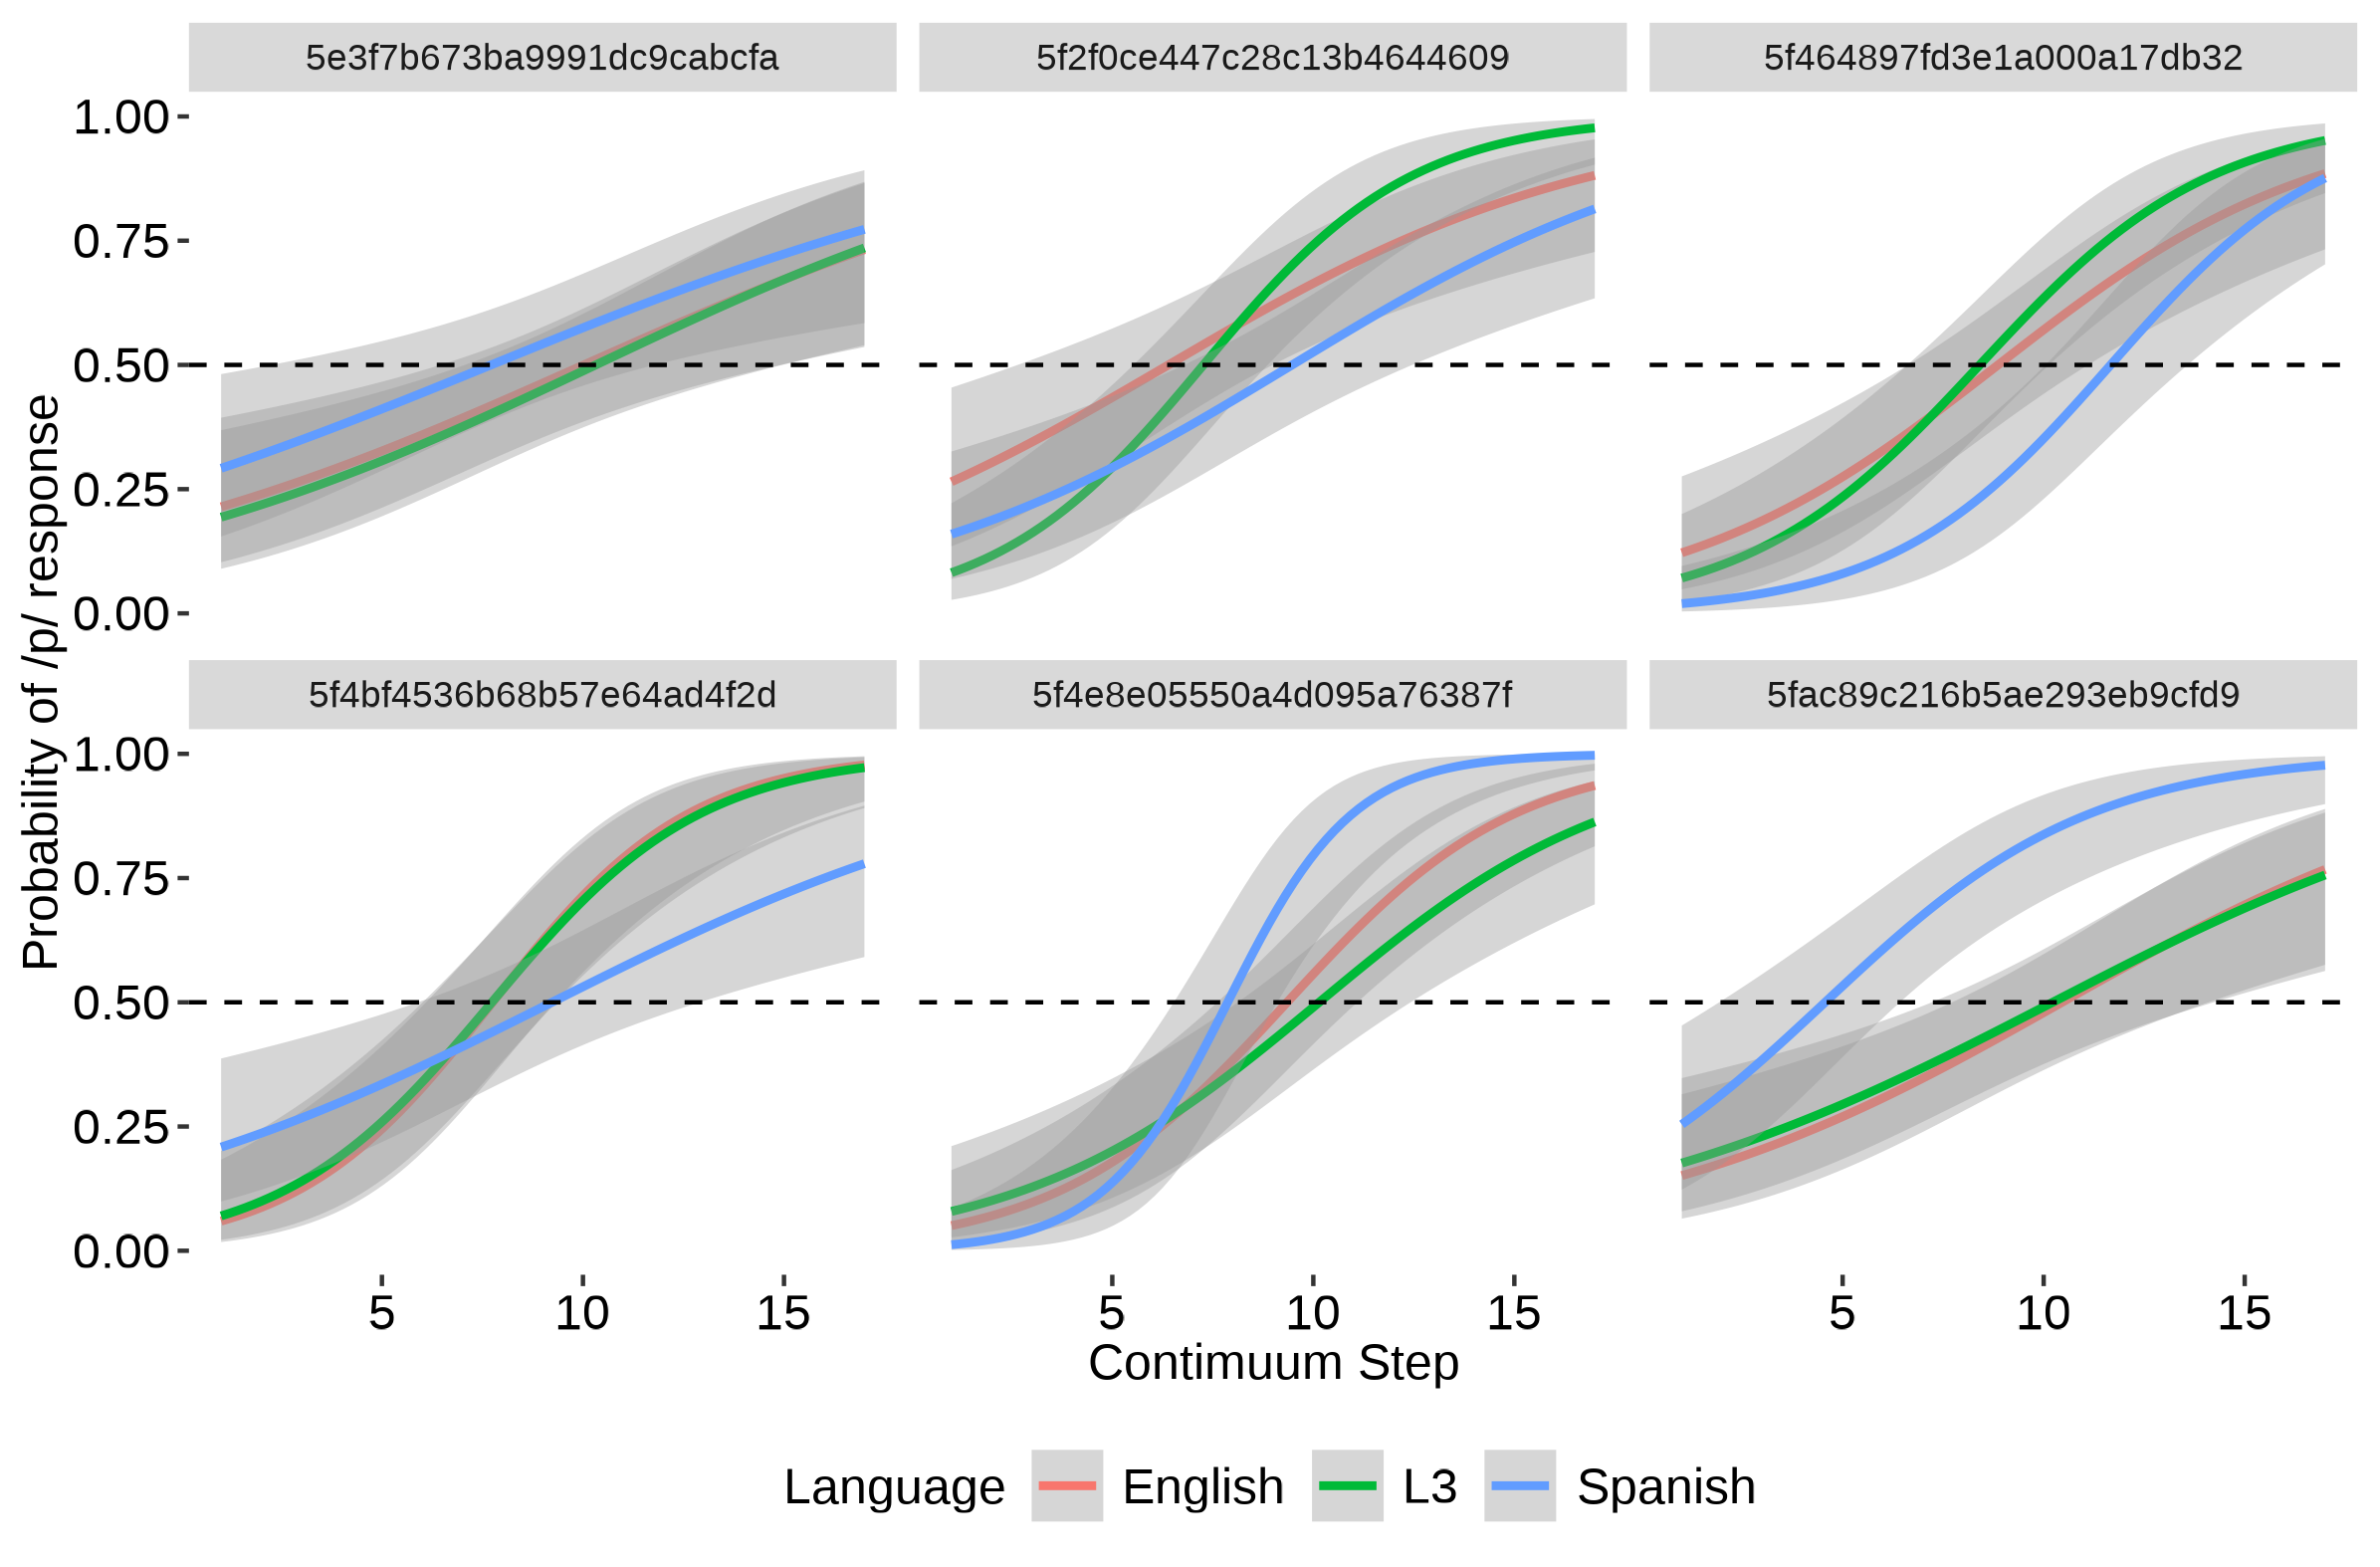
\includegraphics[width=425px]{new_docs/img/dpbe_ppts_eng_ind} \caption{ }\label{fig:unnamed-chunk-9}
\end{figure}

\textbf{Supplementary plots}

N/A participants who had more than one continuum step between both their L3 and L1/L2 and was not intermediate of them both.

\begin{figure}
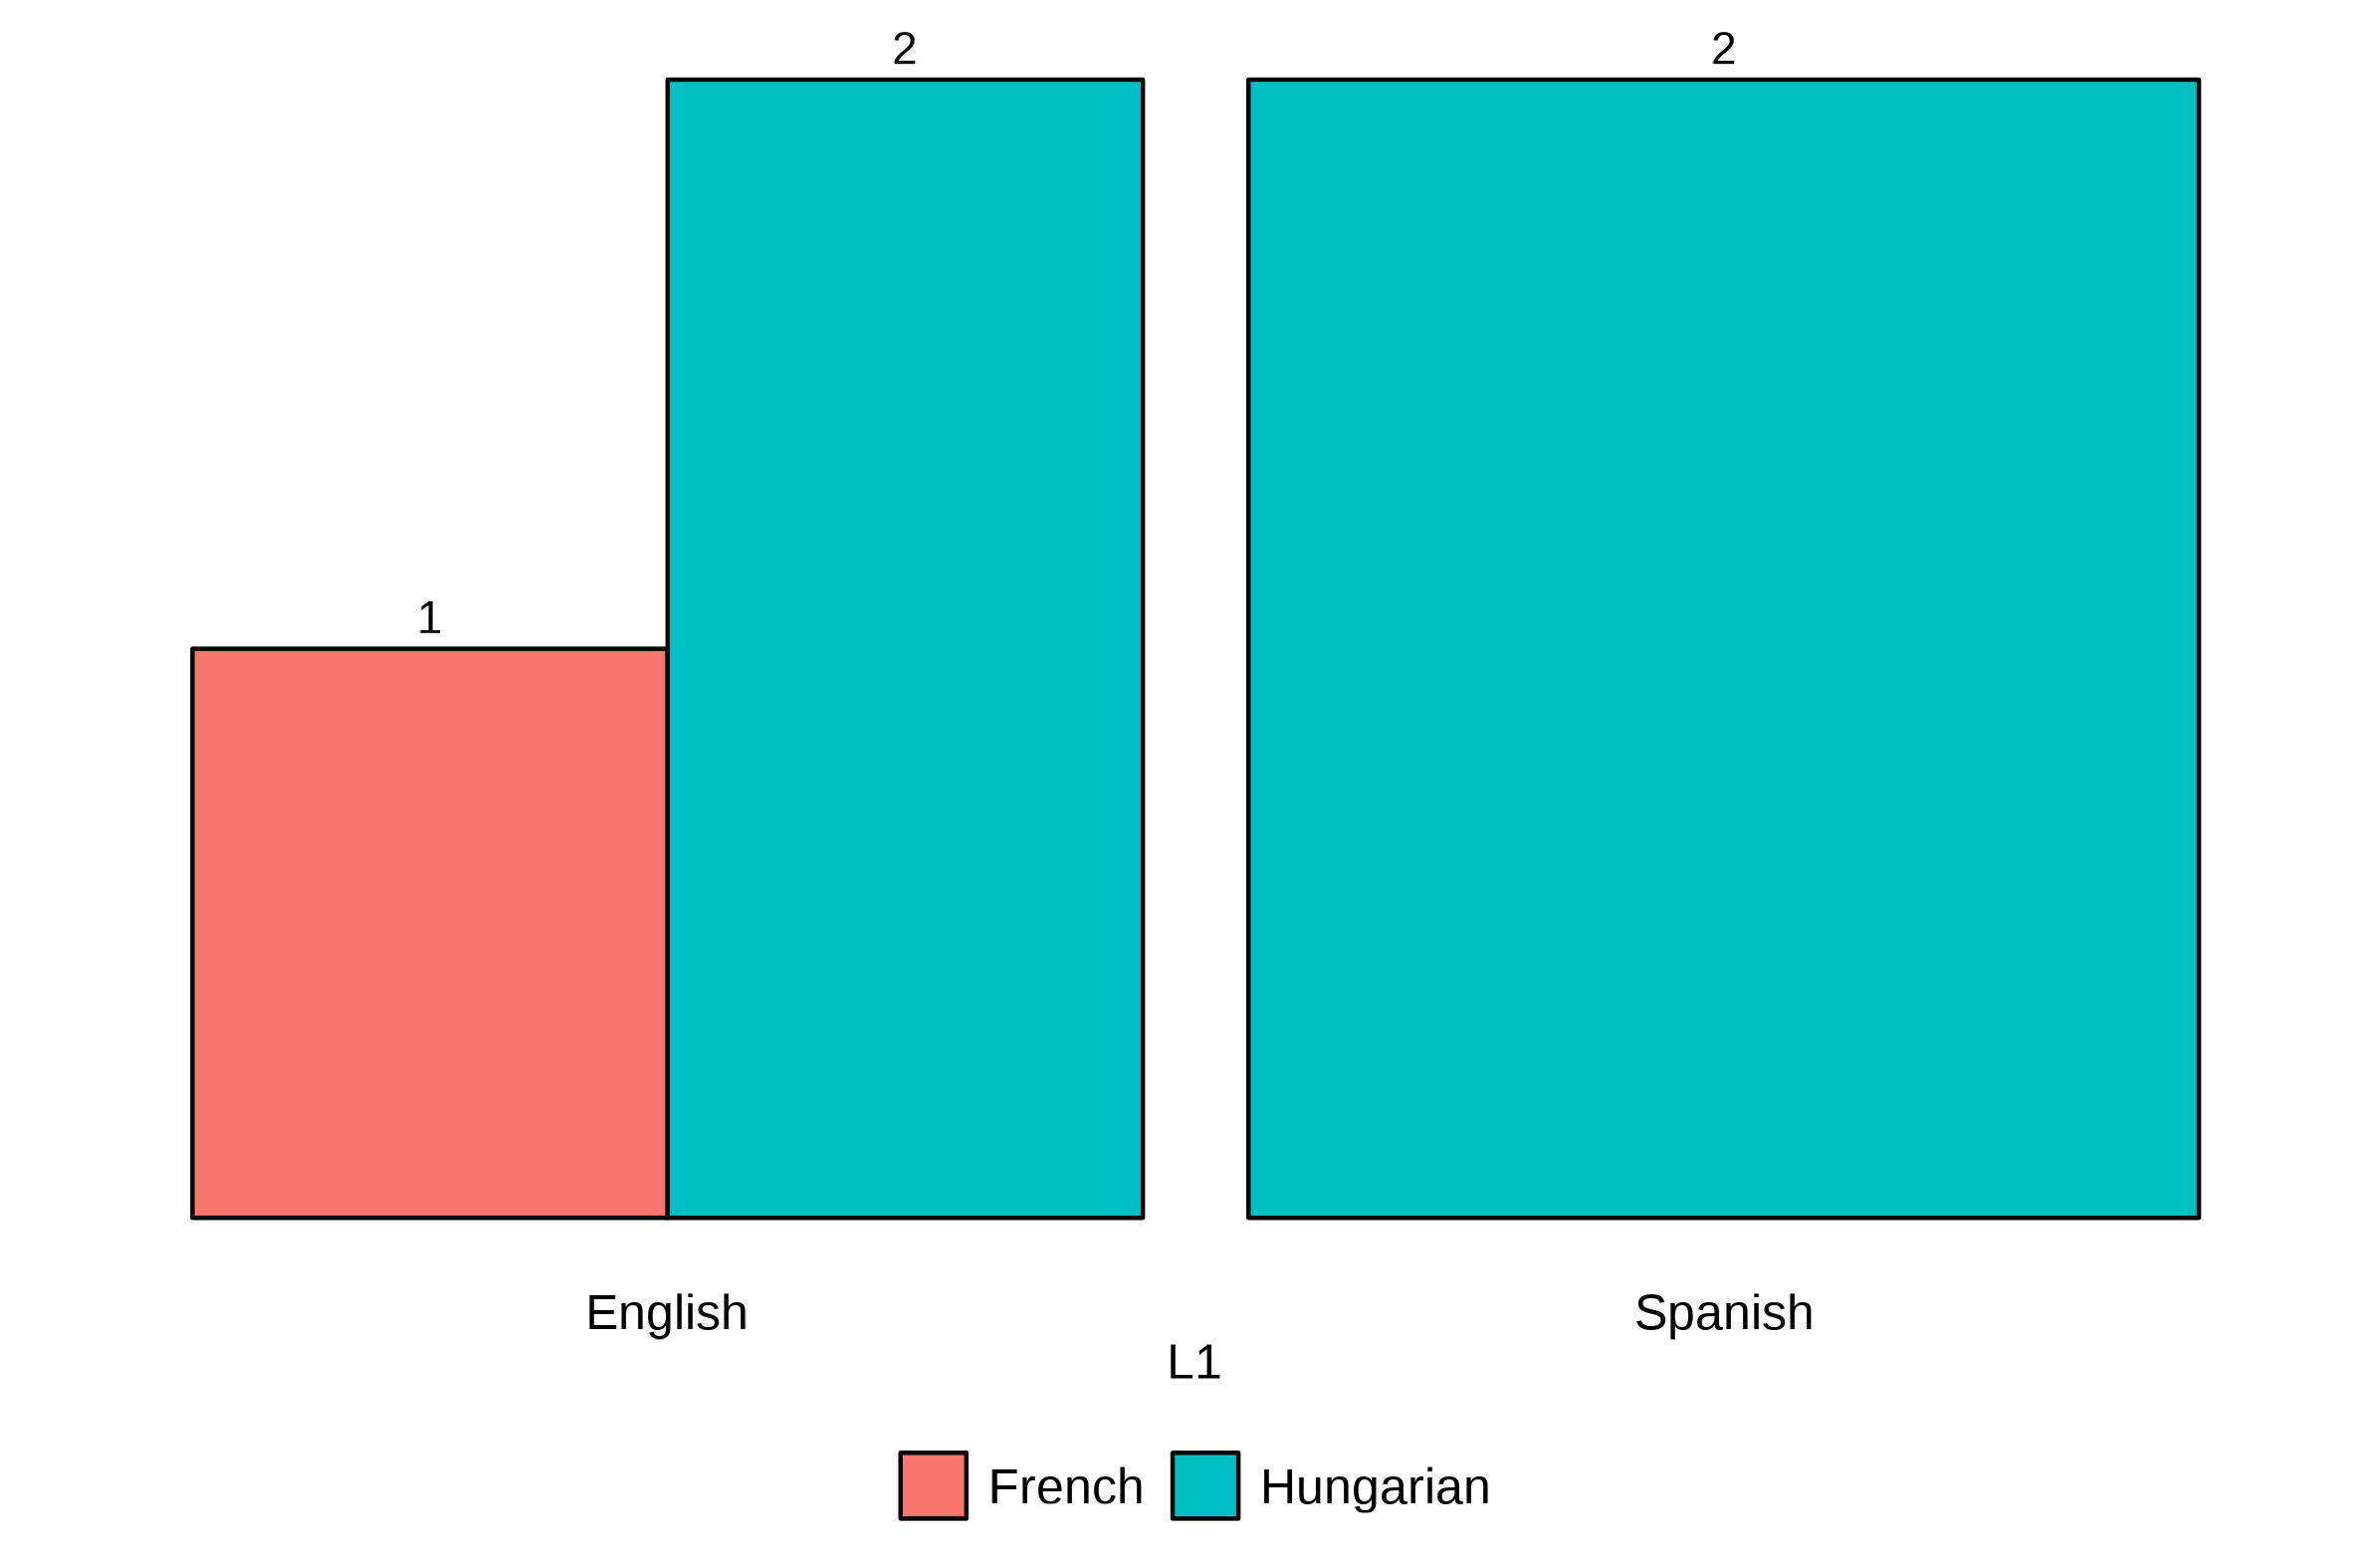
\includegraphics[width=425px]{new_docs/img/na_bar_ppts} \caption{ }\label{fig:unnamed-chunk-10}
\end{figure}
\begin{figure}
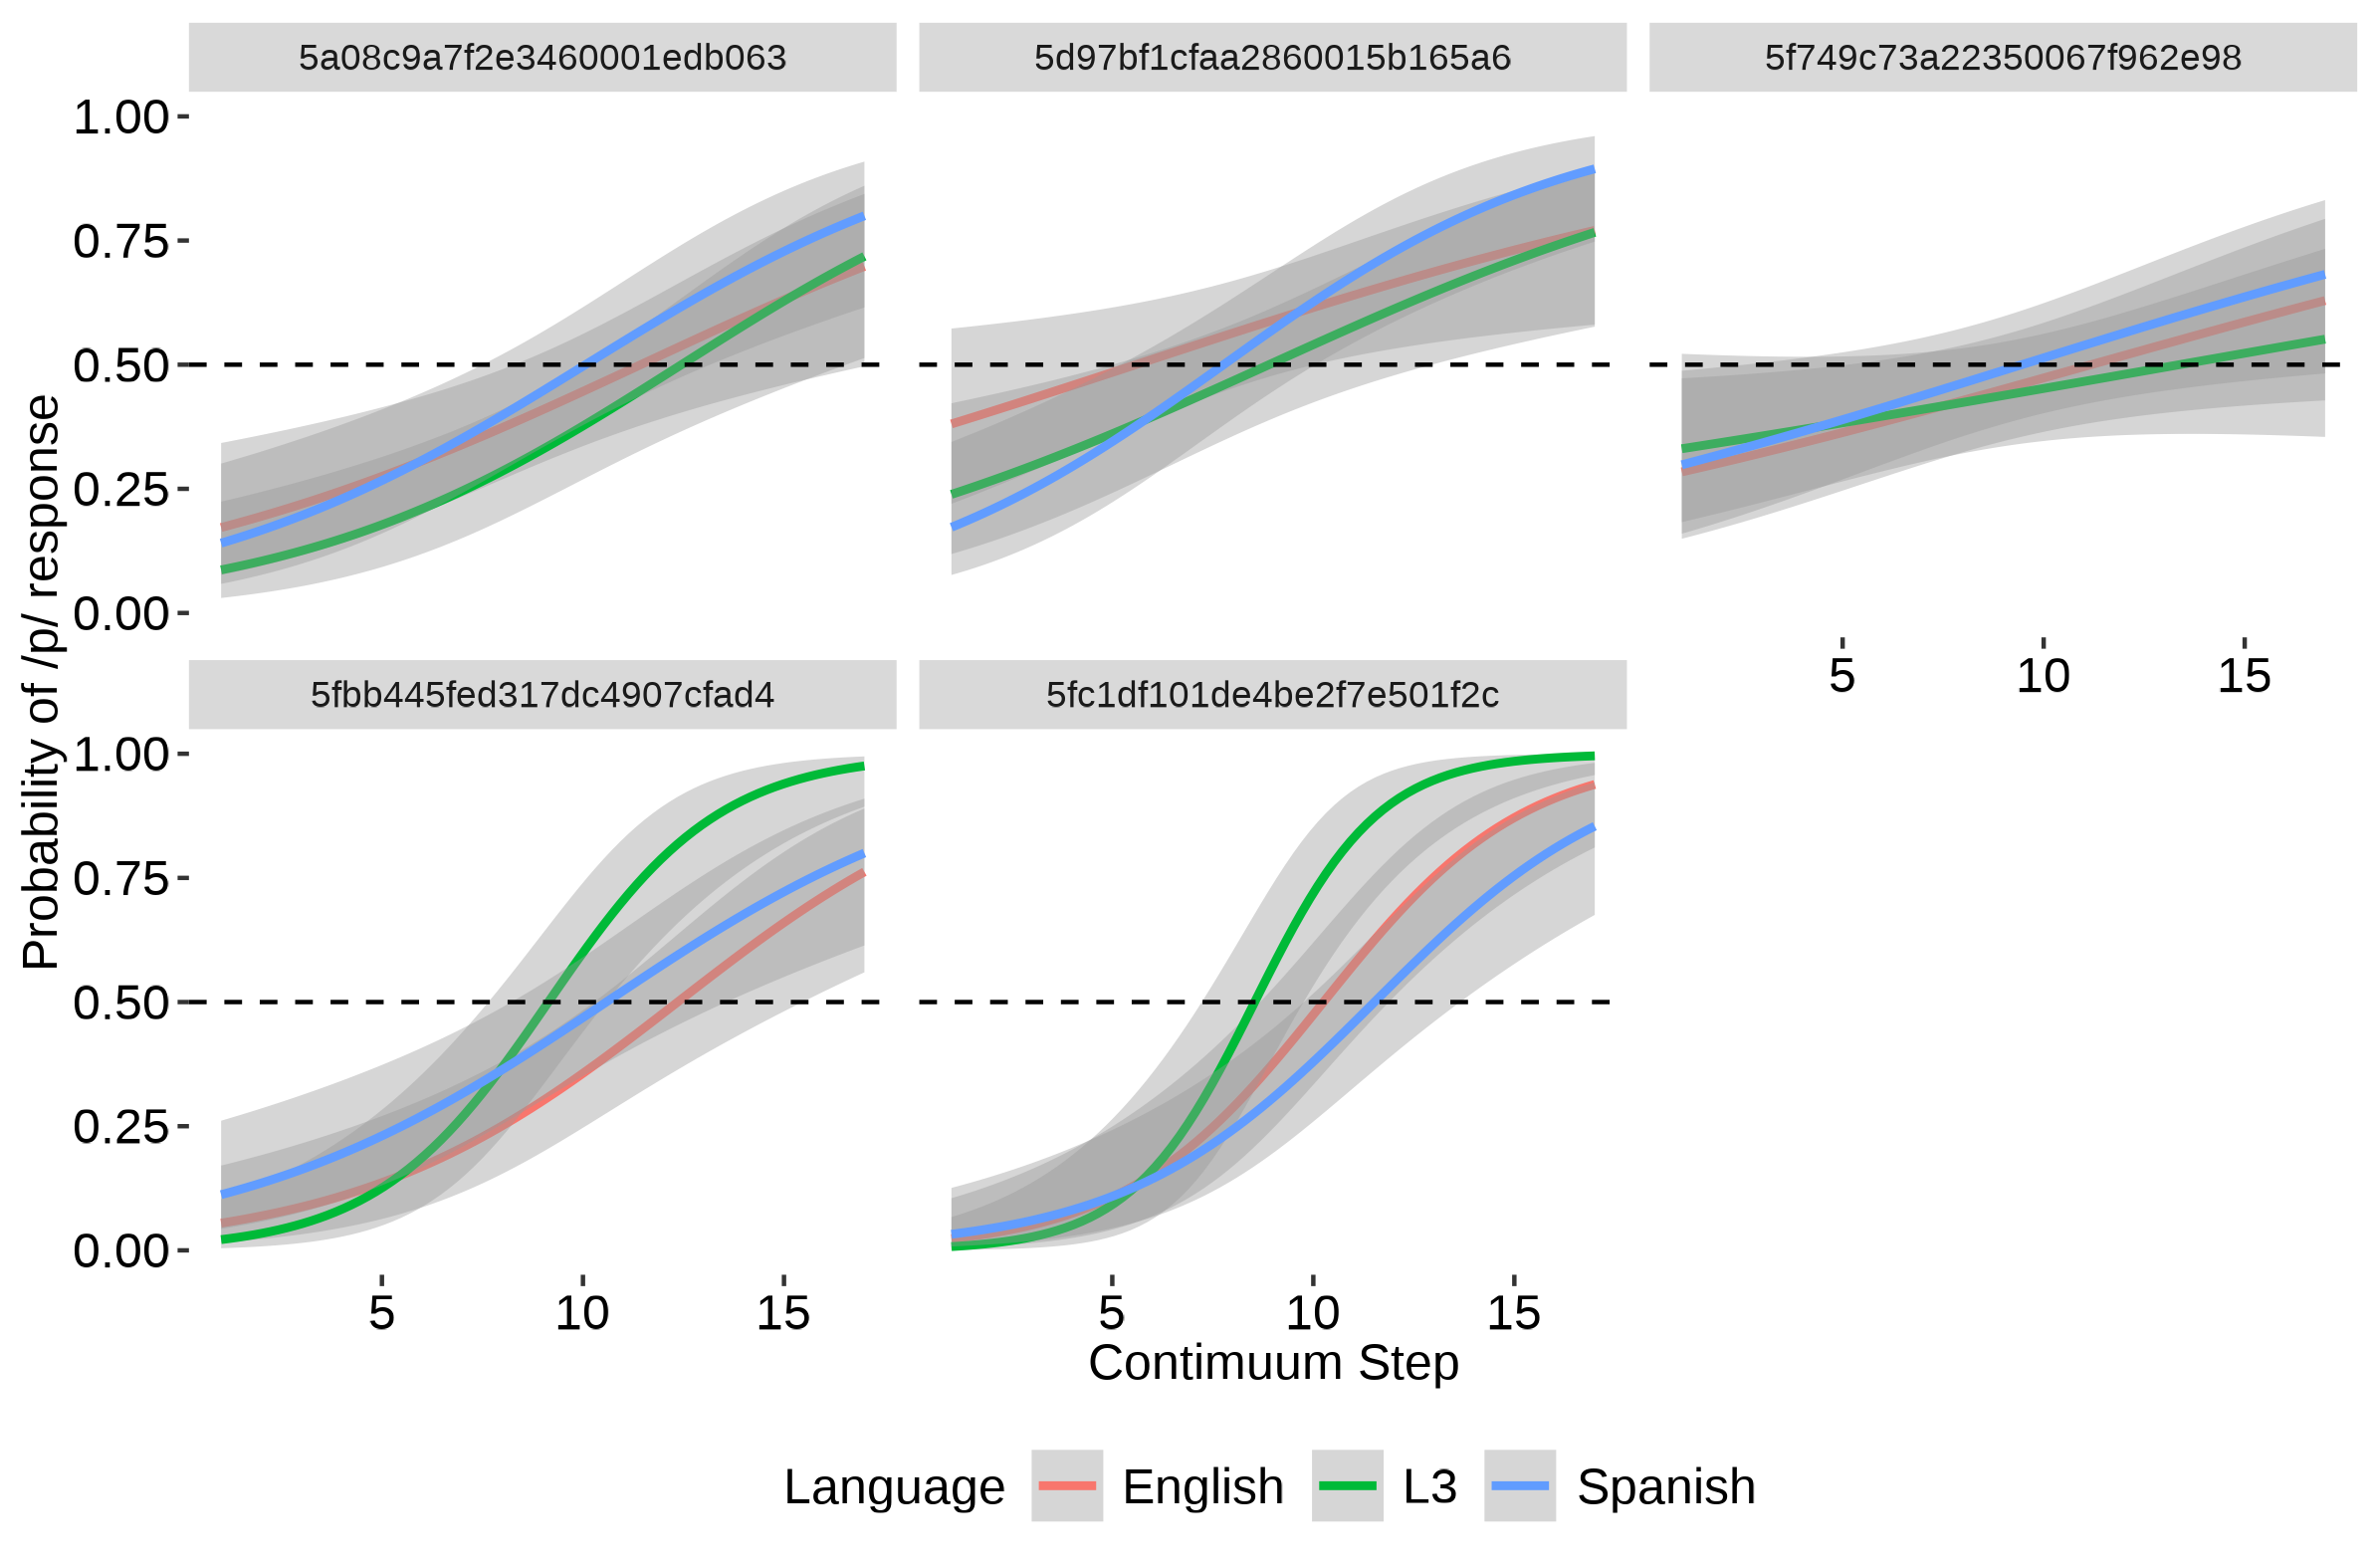
\includegraphics[width=425px]{new_docs/img/na_ppts_s} \caption{ }\label{fig:unnamed-chunk-11}
\end{figure}

\hypertarget{discussion}{%
\section{Discussion}\label{discussion}}

\newpage

\hypertarget{references}{%
\section{References}\label{references}}

\hypertarget{refs}{}
\begin{CSLReferences}{1}{0}
\leavevmode\vadjust pre{\hypertarget{ref-cabrelli_amaro_l2_2012}{}}%
Bardel, C., \& Falk, Y. (2012). The L2 status factor and the declarative/procedural distinction. In J. Cabrelli Amaro, S. Flynn, \& J. Rothman (Eds.), \emph{Studies in bilingualism} (Vol. 46, pp. 61--78). John Benjamins Publishing Company. \url{https://doi.org/10.1075/sibil.46.06bar}

\leavevmode\vadjust pre{\hypertarget{ref-bohn_perceptual_1993}{}}%
Bohn, O.-S., \& Flege, J. E. (1993). Perceptual switching in spanish/english bilinguals. \emph{Journal of Phonetics}, \emph{21}(3), 267--290. \url{https://doi.org/10.1016/S0095-4470(19)31339-7}

\leavevmode\vadjust pre{\hypertarget{ref-cabrelli_amaro_investigating_2016}{}}%
Cabrelli Amaro, J., \& Wrembel, M. (2016). Investigating the acquisition of phonology in a third language -- a state of the science and an outlook for the future. \emph{International Journal of Multilingualism}, \emph{13}(4), 395--409. \url{https://doi.org/10.1080/14790718.2016.1217601}

\leavevmode\vadjust pre{\hypertarget{ref-caramazza_voice_1974}{}}%
Caramazza, A., \& Yeni-Komshian, G. H. (1974). Voice onset time in two french dialects. \emph{Journal of Phonetics}, \emph{2}(3), 239--245. \url{https://doi.org/10.1016/S0095-4470(19)31274-4}

\leavevmode\vadjust pre{\hypertarget{ref-caramazza_bilingual_1974}{}}%
Caramazza, A., Yeni-Komshian, G., \& Zurif, E. B. (1974). Bilingual switching: The phonological level. \emph{Canadian Journal of Psychology/Revue Canadienne de Psychologie}, \emph{28}(3), 310--318. \url{https://doi.org/10.1037/h0081997}

\leavevmode\vadjust pre{\hypertarget{ref-caramazza_acquisition_1973}{}}%
Caramazza, A., Yeni‐Komshian, G. H., Zurif, E. B., \& Carbone, E. (1973). The acquisition of a new phonological contrast: The case of stop consonants in french‐english bilinguals. \emph{The Journal of the Acoustical Society of America}, \emph{54}(2), 421--428. \url{https://doi.org/10.1121/1.1913594}

\leavevmode\vadjust pre{\hypertarget{ref-casillas_perceptual_2018}{}}%
Casillas, J. V., \& Simonet, M. (2018). Perceptual categorization and bilingual language modes: Assessing the double phonemic boundary in early and late bilinguals. \emph{Journal of Phonetics}, \emph{71}, 51--64. \url{https://doi.org/10.1016/j.wocn.2018.07.002}

\leavevmode\vadjust pre{\hypertarget{ref-elman_perceptual_1977}{}}%
Elman, J. L., Diehl, R. L., \& Buchwald, S. E. (1977). Perceptual switching in bilinguals. \emph{The Journal of the Acoustical Society of America}, \emph{62}(4), 971--974. \url{https://doi.org/10.1121/1.381591}

\leavevmode\vadjust pre{\hypertarget{ref-flege_cross-language_1987}{}}%
Flege, J. E., \& Eefting, W. (1987). Cross-language switching in stop consonant perception and production by dutch speakers of english. \emph{Speech Communication}, \emph{6}(3), 185--202. \url{https://doi.org/10.1016/0167-6393(87)90025-2}

\leavevmode\vadjust pre{\hypertarget{ref-garcia-sierra_testing_2009}{}}%
Garcia-Sierra, A., Diehl, R. L., \& Champlin, C. (2009). Testing the double phonemic boundary in bilinguals. \emph{Speech Communication}, \emph{51}(4), 369--378. \url{https://doi.org/10.1016/j.specom.2008.11.005}

\leavevmode\vadjust pre{\hypertarget{ref-gonzales_how_2019}{}}%
Gonzales, K., Byers-Heinlein, K., \& Lotto, A. J. (2019). How bilinguals perceive speech depends on which language they think they're hearing. \emph{Cognition}, \emph{182}, 318--330.

\leavevmode\vadjust pre{\hypertarget{ref-gonzales_bafri_2013}{}}%
Gonzales, K., \& Lotto, A. J. (2013). A \emph{bafri} , un \emph{pafri}: Bilinguals' pseudoword identifications support language-specific phonetic systems. \emph{Psychological Science}, \emph{24}(11), 2135--2142. \url{https://doi.org/10.1177/0956797613486485}

\leavevmode\vadjust pre{\hypertarget{ref-grosjean_neurolinguists_1989}{}}%
Grosjean, F. (1989). Neurolinguists, beware! The bilingual is not two monolinguals in one person. \emph{Brain and Language}, \emph{36}(1), 3--15. \url{https://doi.org/10.1016/0093-934X(89)90048-5}

\leavevmode\vadjust pre{\hypertarget{ref-hazan_perception_1993}{}}%
Hazan, V. L., \& Boulakia, G. (1993). Perception and production of a voicing contrast by french-english bilinguals. \emph{Language and Speech}, \emph{36}(1), 17--38. \url{https://doi.org/10.1177/002383099303600102}

\leavevmode\vadjust pre{\hypertarget{ref-izura_lexical_2016}{}}%
Izura, C., Cuetos, F., \& Brysbaert, M. (2016). \emph{Lexical test for advanced learners of spanish}. American Psychological Association. \url{https://doi.org/10.1037/t47086-000}

\leavevmode\vadjust pre{\hypertarget{ref-lemhofer_lexical_2016}{}}%
Lemhöfer, K., \& Broersma, M. (2016). \emph{Lexical test for advanced learners of english}. American Psychological Association. \url{https://doi.org/10.1037/t47085-000}

\leavevmode\vadjust pre{\hypertarget{ref-li_language_2020}{}}%
Li, P., Zhang, F., Yu, A., \& Zhao, X. (2020). Language history questionnaire ({LHQ}3): An enhanced tool for assessing multilingual experience. \emph{Bilingualism: Language and Cognition}, \emph{23}(5), 938--944. \url{https://doi.org/10.1017/S1366728918001153}

\leavevmode\vadjust pre{\hypertarget{ref-lisker_cross-language_1964}{}}%
Lisker, L., \& Abramson, A. S. (1964). A cross-language study of voicing in initial stops: Acoustical measurements. \emph{\emph{WORD}}, \emph{20}(3), 384--422. \url{https://doi.org/10.1080/00437956.1964.11659830}

\leavevmode\vadjust pre{\hypertarget{ref-lozano-arguelles_conceptually_2020}{}}%
Lozano-Argüelles, C., Fernández Arroyo, L., Rodríguez, N., Durand López, E. M., Garrido Pozú, J. J., Markovits, J., Varela, J. P., Rocafiguera, N. de, \& Casillas, J. V. (2020). {CONCEPTUALLY} {CUED} {PERCEPTUAL} {CATEGORIZATION} {IN} {ADULT} L2 {LEARNERS}. \emph{Studies in Second Language Acquisition}, 1--16. \url{https://doi.org/10.1017/S0272263120000273}

\leavevmode\vadjust pre{\hypertarget{ref-peirce_psychopy2_2019}{}}%
Peirce, J., Gray, J. R., Simpson, S., MacAskill, M., Höchenberger, R., Sogo, H., Kastman, E., \& Lindeløv, J. K. (2019). {PsychoPy}2: Experiments in behavior made easy. \emph{Behavior Research Methods}, \emph{51}(1), 195--203. \url{https://doi.org/10.3758/s13428-018-01193-y}

\leavevmode\vadjust pre{\hypertarget{ref-R-base}{}}%
R Core Team. (2020). \emph{R: A language and environment for statistical computing}. R Foundation for Statistical Computing. \url{https://www.R-project.org/}

\leavevmode\vadjust pre{\hypertarget{ref-rothman_linguistic_2015}{}}%
Rothman, J. (2015). Linguistic and cognitive motivations for the typological primacy model ({TPM}) of third language (L3) transfer: Timing of acquisition and proficiency considered. \emph{Bilingualism: Language and Cognition}, \emph{18}(2), 179--190. \url{https://doi.org/10.1017/S136672891300059X}

\leavevmode\vadjust pre{\hypertarget{ref-simonet_phonetics_2016}{}}%
Simonet, M. (2016). \emph{The phonetics and phonology of bilingualism} (Vol. 1). Oxford University Press. \url{https://doi.org/10.1093/oxfordhb/9780199935345.013.72}

\leavevmode\vadjust pre{\hypertarget{ref-slabakova_scalpel_2017}{}}%
Slabakova, R. (2017). The scalpel model of third language acquisition. \emph{International Journal of Bilingualism}, \emph{21}(6), 651--665. \url{https://doi.org/10.1177/1367006916655413}

\leavevmode\vadjust pre{\hypertarget{ref-westergaard_crosslinguistic_2017}{}}%
Westergaard, M., Mitrofanova, N., Mykhaylyk, R., \& Rodina, Y. (2017). Crosslinguistic influence in the acquisition of a third language: The linguistic proximity model. \emph{International Journal of Bilingualism}, \emph{21}(6), 666--682. \url{https://doi.org/10.1177/1367006916648859}

\leavevmode\vadjust pre{\hypertarget{ref-williams_perception_1977}{}}%
Williams, L. (1977). The perception of stop consonant voicing by spanish-english bilinguals. \emph{Perception \& Psychophysics}, \emph{21}(4), 289--297. \url{https://doi.org/10.3758/BF03199477}

\end{CSLReferences}


\end{document}
